%%%%%%%%%%%%%%%%%%%%%%%%%%%%%%%%%%%%%%%%%%%%%%%%%%%%%%%%%%%%%%%%%%%%%%
% Create report using UT dissertation style
%%%%%%%%%%%%%%%%%%%%%%%%%%%%%%%%%%%%%%%%%%%%%%%%%%%%%%%%%%%%%%%%%%%%%%
\documentclass[12pt]{report}
\usepackage{utdiss2}


%%%%%%%%%%%%%%%%%%%%%%%%%%%%%%%%%%%%%%%%%%%%%%%%%%%%%%%%%%%%%%%%%%%%%%
% Load the necessary packages
%%%%%%%%%%%%%%%%%%%%%%%%%%%%%%%%%%%%%%%%%%%%%%%%%%%%%%%%%%%%%%%%%%%%%%
\usepackage{amsmath,amsthm,amsfonts,amscd}
\usepackage{eucal}
\usepackage{verbatim}
\usepackage{makeidx}
\usepackage{epsfig}
\usepackage{cite}
\usepackage{url}
\usepackage[version=4]{mhchem}

\usepackage[english]{babel}
\usepackage{blindtext}

%%%%%%%%%%%%%%%%%%%%%%%%%%%%%%%%%%%%%%%%%%%%%%%%%%%%%%%%%%%%%%%%%%%%%%
% Required personal information
%%%%%%%%%%%%%%%%%%%%%%%%%%%%%%%%%%%%%%%%%%%%%%%%%%%%%%%%%%%%%%%%%%%%%%
\author{Colin Tan Sullender}
\address{}
\title{Writing a Doctoral Dissertation with \LaTeX{} at
		the University of Texas at Austin}


%%%%%%%%%%%%%%%%%%%%%%%%%%%%%%%%%%%%%%%%%%%%%%%%%%%%%%%%%%%%%%%%%%%%%%
% Required degree and dissertation information
%%%%%%%%%%%%%%%%%%%%%%%%%%%%%%%%%%%%%%%%%%%%%%%%%%%%%%%%%%%%%%%%%%%%%%
\previousdegrees{Ph.D.}
\graduationmonth{August}
\graduationyear{2018}
\typist{the author}


%%%%%%%%%%%%%%%%%%%%%%%%%%%%%%%%%%%%%%%%%%%%%%%%%%%%%%%%%%%%%%%%%%%%%%
% Define names of supervisor(s) and committee members
%%%%%%%%%%%%%%%%%%%%%%%%%%%%%%%%%%%%%%%%%%%%%%%%%%%%%%%%%%%%%%%%%%%%%%
\supervisor
	{Andrew K. Dunn}

\committeemembers
    [Theresa A. Jones]
    [Chong Xie]
    [James W. Tunnell]
    {Ming-Chieh Ding}


%%%%%%%%%%%%%%%%%%%%%%%%%%%%%%%%%%%%%%%%%%%%%%%%%%%%%%%%%%%%%%%%%%%%%%
% Some optional commands to change the document's defaults.	     %
%%%%%%%%%%%%%%%%%%%%%%%%%%%%%%%%%%%%%%%%%%%%%%%%%%%%%%%%%%%%%%%%%%%%%%
%
%\singlespacing
%\oneandonehalfspacing

%\singlespacequote
\oneandonehalfspacequote

\topmargin 0.125in	% Adjust this value if the PostScript file output
			% of your dissertation has incorrect top and
			% bottom margins. Print a copy of at least one
			% full page of your dissertation (not the first
			% page of a chapter) and measure the top and
			% bottom margins with a ruler. You must have
			% a top margin of 1.5" and a bottom margin of
			% at least 1.25". The page numbers must be at
			% least 1.00" from the bottom of the page.
			% If the margins are not correct, adjust this
			% value accordingly and re-compile and print again.
			%
			% The default value is 0.125"

		% If you want to adjust other margins, they are in the
		% utdiss2-nn.sty file near the top. If you are using
		% the shell script Makediss on a Unix/Linux system, make
		% your changes in the utdiss2-nn.sty file instead of
		% utdiss2.sty because Makediss will overwrite any changes
		% made to utdiss2.sty.

%%%%%%%%%%%%%%%%%%%%%%%%%%%%%%%%%%%%%%%%%%%%%%%%%%%%%%%%%%%%%%%%%%%%%%
% Some optional commands to be tested.				     %
%%%%%%%%%%%%%%%%%%%%%%%%%%%%%%%%%%%%%%%%%%%%%%%%%%%%%%%%%%%%%%%%%%%%%%

% If there are 10 or more sections, 10 or more subsections for a section,
% etc., you need to make an adjustment to the Table of Contents with the
% command \longtocentry.
%
%\longtocentry



%%%%%%%%%%%%%%%%%%%%%%%%%%%%%%%%%%%%%%%%%%%%%%%%%%%%%%%%%%%%%%%%%%%%%%
%	Some math support.					     %
%%%%%%%%%%%%%%%%%%%%%%%%%%%%%%%%%%%%%%%%%%%%%%%%%%%%%%%%%%%%%%%%%%%%%%
%
%	Theorem environments (these need the amsthm package)
%
%% \theoremstyle{plain} %% This is the default

\newtheorem{thm}{Theorem}[section]
\newtheorem{cor}[thm]{Corollary}
\newtheorem{lem}[thm]{Lemma}
\newtheorem{prop}[thm]{Proposition}
\newtheorem{ax}{Axiom}

\theoremstyle{definition}
\newtheorem{defn}{Definition}[section]

\theoremstyle{remark}
\newtheorem{rem}{Remark}[section]
\newtheorem*{notation}{Notation}

%\numberwithin{equation}{section}


%%%%%%%%%%%%%%%%%%%%%%%%%%%%%%%%%%%%%%%%%%%%%%%%%%%%%%%%%%%%%%%%%%%%%%
%	Macros.							     %
%%%%%%%%%%%%%%%%%%%%%%%%%%%%%%%%%%%%%%%%%%%%%%%%%%%%%%%%%%%%%%%%%%%%%%
%
%	Here some macros that are needed in this document:

\newcommand{\latexe}{{\LaTeX\kern.125em2%
                      \lower.5ex\hbox{$\varepsilon$}}}

\newcommand{\amslatex}{\AmS-\LaTeX{}}

\chardef\bslash=`\\	% \bslash makes a backslash (in tt fonts)
			%	p. 424, TeXbook

\newcommand{\cn}[1]{\texttt{\bslash #1}}

\makeatletter		% Starts section where @ is considered a letter
			% and thus may be used in commands.
\def\square{\RIfM@\bgroup\else$\bgroup\aftergroup$\fi
  \vcenter{\hrule\hbox{\vrule\@height.6em\kern.6em\vrule}%
                                              \hrule}\egroup}

\makeatother		% Ends sections where @ is considered a letter.
			% Now @ cannot be used in commands.

\makeindex    % Make the index

%%%%%%%%%%%%%%%%%%%%%%%%%%%%%%%%%%%%%%%%%%%%%%%%%%%%%%%%%%%%%%%%%%%%%%
% BEGIN DOCUMENT
%%%%%%%%%%%%%%%%%%%%%%%%%%%%%%%%%%%%%%%%%%%%%%%%%%%%%%%%%%%%%%%%%%%%%%
\begin{document}

\copyrightpage      % Produces the copyright page
\commcertpage       % Produces the doctoral Committee Certification of Approved Version page
\titlepage          % Produces the title page


%%%%%%%%%%%%%%%%%%%%%%%%%%%%%%%%%%%%%%%%%%%%%%%%%%%%%%%%%%%%%%%%%%%%%%
% Dedication and Acknowledgements
%%%%%%%%%%%%%%%%%%%%%%%%%%%%%%%%%%%%%%%%%%%%%%%%%%%%%%%%%%%%%%%%%%%%%%
\begin{dedication}
To my family, friends, and teachers.
\end{dedication}


\begin{acknowledgments}
I wish to thank the multitudes of people who helped me. Time would
fail me to tell of \ldots
\end{acknowledgments}


%%%%%%%%%%%%%%%%%%%%%%%%%%%%%%%%%%%%%%%%%%%%%%%%%%%%%%%%%%%%%%%%%%%%%%
% Abstract
%%%%%%%%%%%%%%%%%%%%%%%%%%%%%%%%%%%%%%%%%%%%%%%%%%%%%%%%%%%%%%%%%%%%%%
\utabstract
\indent
This document has the form of a ``fake'' doctoral dissertation in order to provide an example of such, but it is actually a
copy of Miguel Lerma's documentation for the Mathematics Department Computer Seminar of 25 March 1998 updated in July 2001
and following by Craig McCluskey to meet the March 2001 requirements of the Graduate School.


%%%%%%%%%%%%%%%%%%%%%%%%%%%%%%%%%%%%%%%%%%%%%%%%%%%%%%%%%%%%%%%%%%%%%%
% Table of Contents + List of Tables and Figures
%%%%%%%%%%%%%%%%%%%%%%%%%%%%%%%%%%%%%%%%%%%%%%%%%%%%%%%%%%%%%%%%%%%%%%
\tableofcontents
\listoftables
\listoffigures


%%%%%%%%%%%%%%%%%%%%%%%%%%%%%%%%%%%%%%%%%%%%%%%%%%%%%%%%%%%%%%%%%%%%%%
% Begin Document Body
%%%%%%%%%%%%%%%%%%%%%%%%%%%%%%%%%%%%%%%%%%%%%%%%%%%%%%%%%%%%%%%%%%%%%%

% Chapter 1 - Introduction
%%%%%%%%%%%%%%%%%%%%%%%%%%%%%%%%%%%%%%%%%%%%%%%%%%%%%%%%%%%%%%%%%%%%%%%%%%%%%%%
% Chapter 1 - Introduction
%%%%%%%%%%%%%%%%%%%%%%%%%%%%%%%%%%%%%%%%%%%%%%%%%%%%%%%%%%%%%%%%%%%%%%%%%%%%%%%

\chapter{Introduction}

Cerebrovascular diseases such as stroke are the fifth leading cause of death in the United States and the primary cause of chronic adult disability in the Western world \cite{Kochanek:ut}. Almost 800,000 people in the United States suffer a stroke each year with an estimated total medical cost of over \$40 billion \cite{Benjamin:2018gy}. Ischemic strokes represent approximately 87\% of all cases and occur when blood flow to the brain is disrupted by the formation of a thrombosis or embolism. While less prevalent, hemorrhagic strokes are associated with higher mortality rates \cite{Andersen:2009ih} and occur when an aneurysm or blood vessel ruptures in the brain. Patients who seek treatment within the first few hours of symptom onset have drastically improved outcomes compared to those who receive delayed care \cite{Hacke:2004kf}. The only FDA-approved pharmaceutical treatment for an ischemic stroke is recombinant tissue plasminogen activator (tPA), which enzymatically dissolves blood clots after being administered intravenously. However, only about 7\% of ischemic stroke patients ever receive the treatment, because it must be administered within the first three hours after the onset of symptoms \cite{Schwamm:2013bs}. Unless the patient qualifies for a catheter-based mechanical thrombectomy \cite{Smith:2008dd}, there are very few treatment options once the time window for tPA has passed. Chronic management relies upon pharmaceutical prophylaxis with anticoagulants, antihypertensives, and antihyperlipidemic statins, similar to that of other cardiovascular diseases \cite{StrokePreventioninAtrialFibrillationInvestigators:1991fl, TheStrokeCouncil:2004bi, Endres:2005bg}. Physical rehabilitation is often prescribed to help patients improve functional activity through residual neuroplasticity with varying degrees of efficacy \cite{Jette:2005ii, French:2010ka, Takeuchi:2013ce, French:2016hk}. Current research predominantly focuses on the development of new therapeutics targeting the circulatory and nervous systems through pharmacological, surgical, or behavioral interventions. These preclinical studies have a vital need for quantitative hemodynamic measurements to evaluate the efficacy of interventions in disease models of ischemic stroke.

Focal ischemic stroke is characterized by a localized reduction in blood flow to part of the brain following thrombotic or embolic occlusion of a blood vessel. The loss of blood supply rapidly triggers the ischemic cascade, a series of biochemical events that ultimately cause irreversible tissue damage and neuronal death \cite{Nesto:1987dx}. The region with the most severe reduction in blood flow is termed the "ischemic core" and can experience cellular death within minutes following the occlusion. Surrounding the core is the "ischemic penumbra,"" a region of moderate to minimal ischemia supported by residual perfusion from collateral blood supply. Cellular death proceeds much more slowly in this metastable region as the infarct slowly expands into the penumbra over time \cite{Heiss:1992ge, Ginsberg:1999jy}. This has made the penumbra the primary target for neuroprotective interventions in an attempt to improve tissue viability and restrict the expansion of the core \cite{Felberg:2000gu, RamosCabrer:2011gz}. Understanding the hemodynamic mechanisms and metabolic burdens that affect the evolution of the ischemic penumbra is vital to improving the efficacy of stroke treatments.



%%%%%%%%%%%%%%%%%%%%%%%%%%%%%%%%%%%%%%%%%%%%%%%%%%%%%%%%%%%%%%%%%%%%%%%%%%%%%%%
% Section 1.1 - Imaging of Hemodynamics in the Brain
%%%%%%%%%%%%%%%%%%%%%%%%%%%%%%%%%%%%%%%%%%%%%%%%%%%%%%%%%%%%%%%%%%%%%%%%%%%%%%%
\section{Imaging of Hemodynamics in the Brain}

Modern medical imaging technology has revolutionized our ability to diagnosis and treat pathologies in the human body. Many of these same techniques have also played a critical role in our fundamental understanding of the anatomy and physiology of the brain. Optical imaging modalities have been used extensively \cite{Hillman:2007ep} to study the hemodynamics of phenomena such as neurovascular coupling \cite{Liao:2013jl} and diseases such as stroke \cite{Obrig:2011hy}, epilepsy \cite{Bahar:2006es}, migraines \cite{Bolay:2002jg}, and Alzheimer's \cite{KoronyoHamaoui:2011hk}. However, optical imaging has limited clinical translation because of difficulties in delivering light through the thick, highly-scattering skull. Human hemodynamic studies typically rely upon well-established medical imaging technologies such as magnetic resonance imaging and positron-emission tomography.

%%%%%%%%%%%%%%%%%%%%%%%%%%%%%%%%%%%%%%%%%%%%%%%%%%%%%%%%%%%%%%%%%%%%%%%%%%%%%%%

\subsection{Non-Optical Methods}
The primary clinical technique for studying hemodynamic changes in the brain is magnetic resonance imaging (MRI) \cite{Calamante:2016dg}. MRI has the ability to observe both anatomical structure and localize functional dynamics without the need for exogenous contrast agents. Functional MRI (fMRI) depends upon blood-oxygen-level dependent (BOLD) contrast, which can detect relative changes in the concentration of deoxyhemoglobin, a strongly paramagnetic molecule \cite{Glover:2011eo}. The BOLD hemodynamic response reveals localized recruitment of oxygen via neurovascular coupling and gives fMRI the ability to measure the cerebral metabolic rate of oxygen consumption (\ce{CMRO2}), a metric correlated with brain activity. It also provides an indirect measure of cerebral blood flow (CBF) because \ce{CMRO2} is dependent upon blood flow. However, fMRI suffers from poor spatial and temporal resolutions, prohibiting it from examining neurovascular structure or hemodynamics in fine detail \cite{Glover:2011eo}.

Positron-emission tomography (PET) offers functional localization with high sensitivity at similar resolutions to fMRI but requires the injection or inhalation of a radioactive tracer \cite{Wintermark:2005dd}. CBF and \ce{CMRO2} can be measured using isotopes of oxygen gas or carbon dioxide while the cerebral metabolic rate of glucose consumption (CMRGlc), another proxy for brain activity, can be measured using \ce{^18F} fluorodeoxyglucose (FDG). PET requires access to cyclotron-produced radiopharmaceuticals and the instrumentation is rarely found outside of medical facilities. Radiation exposure also limits the number of successive imaging sessions that can be conducted in a subject.

Transcranial Doppler ultrasound offers measurements of cerebral blood flow velocity in large arteries and veins and is an increasingly popular diagnostic and therapeutic monitoring tool \cite{Sarkar:2007fk}. Combined with anatomical information to obtain vessel size, the velocity measurements can be converted to volumetric flow. Clinically, the technique is limited to diagnosing global or hemispheric hypoperfusion because measurements are constrained to only the largest vessels \cite{Naqvi:2013hd}. However, the temporal resolution is significantly higher than fMRI or PET, which allows for dynamic monitoring of blood flow velocity over time.

%%%%%%%%%%%%%%%%%%%%%%%%%%%%%%%%%%%%%%%%%%%%%%%%%%%%%%%%%%%%%%%%%%%%%%%%%%%%%%%

\subsection{Optical Methods}
Optical imaging offers significantly higher spatial and temporal resolutions but with limited depth penetration compared to non-optical techniques. The increased resolution has facilitated the study of microscale brain hemodynamics and the complex relationship between neural activity and blood flow. However, spatial resolution is highly dependent upon gaining optical access to the area of interest, especially when imaging through highly-scattering tissues such as the skull. In animal models, the surgical implantation of optically-clear cranial windows is a common method to gain direct optical access to surface of the brain.

Pulse oximetry to measure peripheral oxygen saturation (\ce{SO2}) is the most common clinical application of optical hemodynamic imaging. The non-invasive spectroscopic technique is based on absorption differences between oxygenated and deoxygenated hemoglobin and therefore requires no exogenous contrast agents. Transcranial near-infrared spectroscopy (NIRS) is a related technique that has been applied to visualizing functional \cite{Cui:2011en} and ischemic \cite{Murkin:2009eb} cerebral hemodynamics in humans. While it has limited clinical implementations \cite{Hoshi:2011gr}, results from NIRS have been strongly correlated with fMRI measurements in stroke patients \cite{Kato:2002ka}.

Hemoglobin has also been targeted as an endogenous contrast agent for optical intrinsic signal (OIS) imaging and multispectral reflectance imaging. These camera-based approaches measure changes in the reflectance of tissue at multiple wavelengths in order to estimate relative chromophore concentrations \cite{Zepeda:2004hc}. The resulting changes in oxy- and deoxyhemoglobin in response to stimuli are analogous to BOLD contrast from fMRI. OIS imaging has been performed during external stimulation to study the functional organization of the cortex at resolutions much greater than fMRI \cite{Tso:1990ba, Masino:1993tk}. Multispectral imaging has been combined with CBF estimates from laser speckle contrast imaging to measure the metabolic response to focal ischemia \cite{Jones:2008gb}.

Optical imaging can directly measure flow velocities within blood vessels by tracking or labeling erythrocytes. High frame rate cameras can be used for reflectance imaging of hemoglobin within cortical surface vasculature in order to follow erythrocyte motion \cite{Kazmi:2015du}. Alternatively, laser scanning microscopy of fluorescent contrast agents can be used to measure erythrocyte velocity within subsurface microvasculature \cite{Shih:2012bo}. Newer imaging techniques such as optical coherence tomography (OCT), now allow for cross-sectional, depth-resolved measurements of blood flow and hemoglobin concentrations \cite{Srinivasan:2009vx}.



%%%%%%%%%%%%%%%%%%%%%%%%%%%%%%%%%%%%%%%%%%%%%%%%%%%%%%%%%%%%%%%%%%%%%%%%%%%%%%%
% Section 1.2 - Measuring Blood Flow with Dynamic Light Scattering
%%%%%%%%%%%%%%%%%%%%%%%%%%%%%%%%%%%%%%%%%%%%%%%%%%%%%%%%%%%%%%%%%%%%%%%%%%%%%%%
\section{Measuring Blood Flow with Dynamic Light Scattering}

The monitoring of in vivo blood flow dynamics is invaluable in both clinical and laboratory environments for understanding numerous physiological and pathophysiological phenomena. Angiographic techniques and ultrasound have garnered widespread adoption in clinics for providing anatomical and hemodynamic information. Optical imaging using dynamic light scattering (DLS) has become increasingly popular in preclinical research for measuring perfusion and has begun translating to clinical applications. The most common DLS techniques are laser Doppler flowmetry and laser speckle contrast imaging \cite{Briers:2001hy, Dunn:2011gi}. These two modalities are different strategies for imaging the same underlying physical phenomenon and are inherently based upon Doppler shifts in the frequency of coherent light caused by particle motion.

%%%%%%%%%%%%%%%%%%%%%%%%%%%%%%%%%%%%%%%%%%%%%%%%%%%%%%%%%%%%%%%%%%%%%%%%%%%%%%%
\subsection{Laser Doppler Flowmetry}

Laser Doppler flowmetry (LDF) relies upon the frequency spectrum analysis of backscattered coherent light to measure relative perfusion \cite{Briers:2001hy}. While it offers high temporal resolution, LDF is typically limited to measurements at a single spatial location. The introduction of scanning mirrors allow for spatially-resolved measurements at the expense of speed, with low-resolution (256 x 256 pixels) acquisitions taking several minutes in commercially available systems \cite{Rajan:2008di}. Full-field laser Doppler imaging (LDI) offers higher resolutions (480 x 480 pixels) at significantly faster speeds (14 frames per second) but relies upon expensive high frame rate cameras and complex acquisition hardware \cite{Lopez:2011bk}. LDF is frequently used as the "gold standard" during the development of newer DLS flowmetry techniques.

%%%%%%%%%%%%%%%%%%%%%%%%%%%%%%%%%%%%%%%%%%%%%%%%%%%%%%%%%%%%%%%%%%%%%%%%%%%%%%%
\subsection{Laser Speckle Contrast Imaging}

Laser speckle contrast imaging (LSCI) is a full-field optical imaging technique that provides instantaneous maps of blood flow by imaging time-varying laser speckle. The technique was first demonstrated by Fercher and Briers in 1981 using single-exposure photography of retinal blood flow \cite{Fercher:1981jh}. Because images were captured on film and required development prior to processing, the earliest LSCI instruments suffered from very low temporal resolutions and large uncertainties. The arrival of commercially available CCD cameras and faster computers in the 1990s allowed for near real-time LSCI perfusion measurements in the skin \cite{Briers:1995iu, Briers:1996kfa}. The technique was first applied to imaging CBF dynamics in rodents in 2001 \cite{Dunn:2001dj} and has since seen widespread adoption by the neuroscience community for animal studies on stroke \cite{Ayata:2004ba, Strong:2005kj, Armitage:2010ga}, spreading depression \cite{Ayata:2004ck, Shin:2006dc}, and functional activation \cite{Dunn:2005gw, Durduran:2016el}. LSCI has also seen clinical translation as an intraoperative tool for monitoring blood flow and perfusion during brain surgery \cite{Hecht:2009gu, Parthasarathy:2010gh}.

%%%%%%%%%%%%%%%%%%%%%%%%%%%%%%%%%%%%%%%%%%%%%%%%%%%%%%%%%%%%%%%%%%%%%%%%%%%%%%%
\subsubsection{Theory}

Laser speckle is the random interference pattern produced when coherent light scatters from a rough surface or inhomogeneous medium. It manifests because scattered photons travel slightly different path lengths, resulting in constructive and destructive interference between the out of phase coherent light waves. Imaging this scattered light produces a random two-dimensional interference pattern on the detector known as subjective speckle \cite{Ennos:1975et}. If the sample contains scattering particles in motion, such as erythrocytes flowing through vasculature, the speckle pattern will fluctuate temporally. Imaging a time-varying speckle pattern results in the integration of these temporal intensity fluctuations over the camera's exposure time. Assuming the exposure time is longer than the time scale of the speckle intensity fluctuations (\textless1 ms for biological tissues), the resulting speckle pattern will be blurred by the integration. Regions with greater motion will experience more rapid intensity fluctuations and therefore more blurring of the imaged speckle pattern. Because the dynamics of the speckle pattern encodes information about the underlying particle motion, a measure of flow can be obtained by quantifying the spatial blurring. This requires calculating the local speckle contrast ($K$), which is defined as the ratio between the standard deviation ($\sigma_s$) and the mean intensity of pixel values ($\langle{I}\rangle$) within a small region of the image at a single exposure time ($T$) \cite{Briers:1996kfa}.
%
% Equation - Speckle Contrast
\begin{equation}
    \label{eq:speckle_contrast}
    K(T) = \frac{\sigma_s(T)}{\langle{I}\rangle}
\end{equation}

A full speckle contrast image is obtained by computing Equation \ref{eq:speckle_contrast} within an $N$ x $N$ sliding window at every pixel of the raw image. The window size must be chosen carefully to ensure an accurate estimate of local contrast while maintaining adequate spatial resolution in the resulting image. Statistical analysis \cite{Duncan:2008hs} and past precedent \cite{Dunn:2011gi} have established $N = 7$ as an optimal window size and it is used exclusively throughout this dissertation. A properly sampled \cite{Kirkpatrick:2008ke} speckle pattern will produce speckle contrast values ranging between 0 and 1 \cite{Boas:2010vr}. When $K = 1$, there is no blurring of the speckle pattern and therefore no discernible motion in the sample during the camera exposure. However, when $K = 0$, the scattering particles are moving sufficiently fast to average out all the speckles.

% Figure - Simple LSCI Schematic
\begin{figure}
    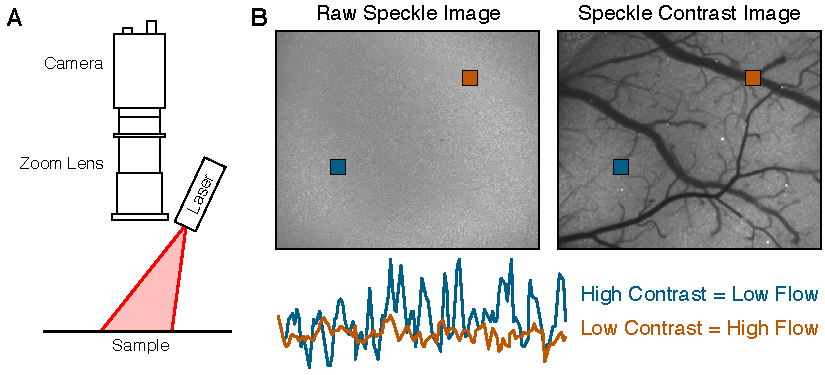
\includegraphics{figures/chapter_1/lsci_schematic.pdf}
    \caption {
        \label{fig:lsci_schematic}
        \textbf{(A)} Traditional LSCI microscope system consisting of an illuminating laser, imaging optics, and a camera. \textbf{(B)} Raw intensity image of the speckle pattern and the resulting speckle contrast image from vasculature in the mouse cerebral cortex. Regions of high contrast in the intensity image (blue) have low flow compared to regions with low contrast (red), which have high flow.
    }
\end{figure}

An example of the raw intensity image of the speckle pattern and corresponding computed speckle contrast image are shown in Figure \ref{fig:lsci_schematic}B. The imagery was obtained \textit{in vivo} from the cerebral cortex of a mouse under general anesthesia. The graininess of the speckle pattern can be seen in the raw intensity image, with some regions appearing more blurred than others. The speckle contrast image was computed directly from the intensity image using Equation \ref{eq:speckle_contrast} to generate a two-dimensional map of motion for the field-of-view. Within the cortex, erythrocytes are the primary moving scattering particles and therefore vasculature is highlighted by the speckle contrast image. Regions of higher flow, such as a large vessel, experience more blurring of the speckle pattern and therefore have lower $K$ values. Conversely, regions of low flow, such as the space between resolvable surface vessels (parenchyma), experience less blurring and therefore have higher $K$ values. Measurements within the parenchyma sample the slower, more isotropic blood flow of unresolvable microvasculature beneath the surface of the cortex.

The shallow depth penetration of LSCI is a significant limitation of the imaging technique. Detected photons only sample a few hundred microns of superficial tissue without any depth resolution and are heavily-weighted towards large surface vasculature \cite{Davis:2014kc}. While skin and retinal imaging can be performed directly on the tissue of interest, CBF imaging requires either thinning or removing the skull to gain optical access \cite{Boas:2010vr}.

%%%%%%%%%%%%%%%%%%%%%%%%%%%%%%%%%%%%%%%%%%%%%%%%%%%%%%%%%%%%%%%%%%%%%%%%%%%%%%%
\subsubsection{Instrumentation}

The simple instrumentation necessary to perform LSCI has contributed to its popularity as a blood flow imaging technique. A basic LSCI microscope consists of an illuminating laser, imaging optics, and a camera (Figure \ref{fig:lsci_schematic}A). The laser output is expanded to broadly epi-illuminate the area of interest at a normal to oblique angle depending on the application. Red to near-infrared laser diodes (600-850 nm) are typically used to take advantage of the tissue optical window where scattering dominates absorption by hemoglobin or water. Because LSCI is based entirely upon scattering, wavelength is less important than other imaging techniques that rely upon absorption. However, the coherence length of the laser dictates the longest possible path length through the tissue that can be properly sampled for quantitative flow information. Lasers with narrow spectral bandwidths (e.g. single longitudinal mode or narrow linewidth lasers) offer coherence lengths of several meters and are more than sufficient for use in LSCI.

Camera selection varies broadly in literature and generally any charge-coupled device (CCD) or complementary metal-oxide-semiconductor (CMOS) camera is appropriate for use with LSCI \cite{Draijer:2008ic, Boas:2010vr}. Even cheap cameras such as webcams have been shown to provide reliable blood flow imagery \cite{Richards:2013bi}. While spectral sensitivity, bit depth, pixel size, frame rate, and noise are all important factors to consider, most researchers use the cameras readily available in their laboratory. However, it is critical that the speckle pattern is properly sampled such that the speckle size is at least twice the size of a single camera pixel \cite{Kirkpatrick:2008ke}. Deviation from the spatial Nyquist sampling criterion will reduce contrast and decrease the variation in the speckle contrast image.

%%%%%%%%%%%%%%%%%%%%%%%%%%%%%%%%%%%%%%%%%%%%%%%%%%%%%%%%%%%%%%%%%%%%%%%%%%%%%%%
\subsubsection{Quantitative Accuracy}

Speckle contrast values are only indicative of the amount of motion in a sample and are not linearly proportional to particle speed or volumetric flow. Understanding the nonlinear relationship with the complex underlying blood flow is an active area of research in the DLS field \cite{Duncan:2008fd, Briers:2013es}. Quantitative flow measurements require accurately relating the speckle contrast value to the characteristic decay time ($\tau_c$) of the speckle autocorrelation function. DLS theory has established that the speckle autocorrelation time is inversely proportional to the speed of the scatters in the single scattering regime \cite{Bonner:1981hga} and weighted by the number of dynamic scattering events under multiple scattering \cite{Boas:1997kf, Kazmi:2015du, Davis:2016ik}. Since Fercher and Briers first proposed a simple model relating $K$ and $\tau_c$ \cite{Fercher:1981jh}, there have been numerous improvements to more robustly extract the flow contributions from the observed speckle \cite{Bandyopadhyay:2005bg, Parthasarathy:2008el}. The model described by Bandyopadhyay, \textit{et al.} \cite{Bandyopadhyay:2005bg} relates the speckle variance ($K^2$) with $\tau_c$ and the camera exposure time ($T$)
%
% Equation - Bandyopadhyay Equation
\begin{equation}
    \label{eq:bandyopadhyay}
    K^2(T,\tau_c) = \beta \frac{e^{-2x} - 1 + 2x}{2x^{2}}
\end{equation}
%
where $x = T/\tau_c$ and $\beta$ is a normalization factor that accounts for speckle averaging due to the mismatch between speckle size and pixel size, polarization, and the finite coherence length of the laser \cite{Lemieux:1999ko}. This model assumes that detected photons only experience single scattering interactions and that the underlying particle motion has a Lorentzian velocity distribution. Despite these assumptions, Equation \ref{eq:bandyopadhyay} has been used extensively to relate measured speckle contrast with relative blood flow \cite{Dunn:2011gi,Boas:2010vr} and will be used throughout this dissertation.

The inverse correlation time (ICT) is frequently interpreted as being proportional to the speed of the moving particles ($1/\tau_c \propto \nu_{scatterers}$) based on assumptions from laser Doppler flowmetry \cite{Bonner:1981hga}. While highly dependent upon the optical properties and flow conditions of the sample, ICT values in single vessels correspond to the speed of the flowing erythrocytes. In parenchyma regions, ICT is a measure of local perfusion because flow cannot be isolated to individual vessels from the integrated contributions of the unresolvable microvasculature \cite{Durduran:2016el, Dunn:2011gi}. Despite these assumptions and limitations, multiple studies have demonstrated strong correlations between LSCI estimates of CBF and absolute measurements from other perfusion indices \cite{Ayata:2004ba, Strong:2005kj, Kazmi:2015du}.



%%%%%%%%%%%%%%%%%%%%%%%%%%%%%%%%%%%%%%%%%%%%%%%%%%%%%%%%%%%%%%%%%%%%%%%%%%%%%%%
% Section 1.3 - Measuring Oxygen Tension In Vivo
%%%%%%%%%%%%%%%%%%%%%%%%%%%%%%%%%%%%%%%%%%%%%%%%%%%%%%%%%%%%%%%%%%%%%%%%%%%%%%%
\section{Measuring Oxygen Tension \textit{In Vivo}}

\textit{In vivo} measurements of molecular oxygen have historically been made using highly invasive Clarke electrodes that are limited to point measurements outside the vascular lumen \cite{Vovenko:1999be, Tsai:2003cc, Roussakis:2015eu}. While targets as small as a few microns can be measured with the appropriate electrode, there are significant tradeoffs between the signal-to-noise ratio and spatial specificity depending on probe size. Electrodes can also only approximate intravascular oxygen concentrations through measurements in nearby interstitial tissue. Magnetic resonance techniques allow for noninvasive imaging of hemoglobin saturation, but suffer from low spatial resolutions and can only be correlated with free oxygen levels in the blood \cite{Roussakis:2015eu, Dunn:2003hg, Hou:2003hb, Liu:2006bt}. Oxygen-sensitive porphyrin probes allow for noninvasive, highly sensitive optical oxygenation measurements based on phosphorescence quenching \cite{Vinogradov:2012tda}. While an injection of the probe is required, absolute oxygen tension (\ce{pO2}) can be directly calculated from the lifetime of the measured phosphorescence decay.

%%%%%%%%%%%%%%%%%%%%%%%%%%%%%%%%%%%%%%%%%%%%%%%%%%%%%%%%%%%%%%%%%%%%%%%%%%%%%%%

\subsection{Oxygen-Dependent Quenching of Phosphorescence}
Recent advances in oxygen-sensitive probe design have made oxygen-dependent quenching of phosphorescence a powerful tool for \textit{in vivo} measurements of \ce{pO2} within both intravascular and interstitial spaces \cite{Vinogradov:2012tda, Esipova:2011hi}. This method relies upon dissolved environmental oxygen quenching the phosphorescence of porphyrin dyes or ruthenium complexes and causing a change in excited state lifetime (Figure \ref{fig:jablonski}A).  The \ce{pO2} can be quantified from the measured lifetime using the Stern-Volmer relationship:
%
% Equation - Stern-Volmer Relationship
\begin{equation}
    \label{eq:stern-volmer}
    \frac{\tau_{0}}{\tau} = 1 + k_{q}\tau_{0}[pO_{2}]
\end{equation}
%
where $\tau$ is the measured phosphorescence lifetime, $\tau_{0}$ is the unquenched lifetime, and $k_{q}$ is a probe-specific quenching rate constant that depends upon the local environment (temperature, pH, atmospheric pressure, and salinity). Equation \ref{eq:stern-volmer} allows for the absolute oxygen tension to be obtained from the measured phosphorescence lifetime provided $k_q$ and $\tau_{0}$ are well-characterized under physiological conditions. Furthermore, because lifetime measurements are independent of absolute intensity, they can easily be isolated from other chromophores and tissue scattering, making them ideal for integration into multi-modal imaging systems.

% Figure - Jablonksi Diagram
\begin{figure}
    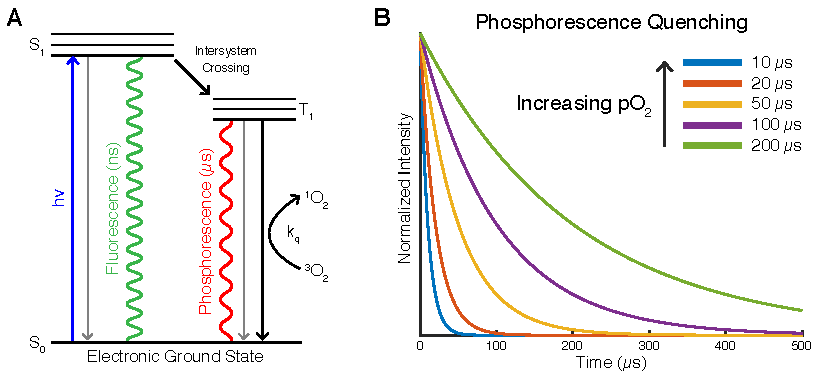
\includegraphics{figures/chapter_1/jablonski.pdf}
    \caption {
        \label{fig:jablonski}
        \textbf{(A)} Jablonski diagram of phosphorescence quenching by environmental molecular oxygen. \textbf{(B)} Phosphorescence quenching causes a reduction in the measured lifetime and is dependent upon [\ce{O2}] or \ce{pO2}.
    }
\end{figure}

The phosphorescence lifetime can be measured in the time domain by exciting the probe with a short pulse of light and collecting the emitted phosphorescence. The resulting phosphorescent decay curve can then be fit to an exponential to obtain the phosphorescence lifetime ($\tau$):
%
% Equation - Exponential Decay
\begin{equation}
    \label{eq:exponential_decay}
    I(t) = A + Be^{-t / \tau}
\end{equation}

Alternatively, frequency domain measurements can be made by calculating the phase angle or modulation depth of the phosphorescence generated by a sinusoidally-modulated laser. While excitation light is utilized more efficiently in frequency domain measurements, they are more difficult to implement than time domain measurements.

Because phosphorescence can be limited to an optical excitation volume, depth-resolved spatial mappings of \ce{pO2} can be acquired \cite{Yaseen:2009ep, Kazmi:2013ey}. Point detectors such as avalanche photodiodes or photomultiplier tubes are commonly used to acquire the phosphorescent decays because of their high sensitivity, gain, and temporal resolutions. \textit{In vivo} measurements of oxygen-dependent quenching of phosphorescence have been conducted in a variety of tissues including the retina, brain, muscle, and peritoneum \cite{Vovenko:1999be}. The technique has also been used extensively to study cortical oxygenation, often in conjunction with other imaging techniques \cite{Yu:2013fd, Devor:2014ke}.



%%%%%%%%%%%%%%%%%%%%%%%%%%%%%%%%%%%%%%%%%%%%%%%%%%%%%%%%%%%%%%%%%%%%%%%%%%%%%%%
% Section 1.4 - Research Overview
%%%%%%%%%%%%%%%%%%%%%%%%%%%%%%%%%%%%%%%%%%%%%%%%%%%%%%%%%%%%%%%%%%%%%%%%%%%%%%%
\section{Research Overview}

The overall goal of this research is the development of an optical imaging platform capable of chronically monitoring cerebral blood flow and oxygen tension in order to better understand cortical hemodynamics during ischemic stroke and the subsequent recovery.


%%%%%%%%%%%%%%%%%%%%%%%%%%%%%%%%%%%%%%%%%%%%%%%%%%%%%%%%%%%%%%%%%%%%%%%%%%%%%%%
% END Chapter 1
%%%%%%%%%%%%%%%%%%%%%%%%%%%%%%%%%%%%%%%%%%%%%%%%%%%%%%%%%%%%%%%%%%%%%%%%%%%%%%%


\chapter{Introduction}
\index{Introduction@\emph{Introduction}}%


This document deals with how to write a doctoral dissertation 
using \LaTeX{}, and how to use the \texttt{utdiss2} package. 
\index{utdiss2 package@{\texttt{utdiss2} package}}%

The latest version of this document/package can be obtained from
\url{http://www.ph.utexas.edu/~laser/craigs_stuff/LaTeX/}.\footnote{I
will be transferring this page to the Office of Graduate
Studies when I graduate. The new URL isn't defined yet, but I will
place a ``redirect'' at this URL to send your browser to the correct
location when the transition occurs.}
If your installation of LaTeX is missing any style files used in this
document (most likely with a \cn{usepackage\{package-name.sty\}}
command at the beginning of disstemplate.tex), take a look at the link
on this page to ``Frequently Requested Style Files'' or on the
Comprehensive TeX Archive Network, \url{http://www.ctan.org}.

In case of any confict between the requirements of the Office of Graduate
Studies and what this document says to do, the requirements of the Office
of Graduate Studies prevail.

\section{History of This Package}
\index{History of This Package@\emph{History of This Package}}%

In 1991 the \texttt{utdiss} package was written by Young U. Ryu 
\index{Young U. Ryu}%
in order to be used in the preamble of \LaTeX{} doctoral dissertation
files at the University of Texas at Austin. 
\index{University of Texas at Austin}%
Since then some changes have occured, the most important one
being the introduction of a new version of \LaTeX{} 
\index{LaTeX@{\LaTeX{}}}%
called \LaTeXe{}. 
\index{LaTeX2e@{\LaTeXe{}}}%

In order to partially adapt the utdiss package to this new version
of \LaTeX{}, Miguel Lerma introduced a few modifications in it,
and his document, \textit{How to Write a Doctoral Dissertation
with \LaTeX{}}, served as a test for it. His new package was
called \texttt{utdiss1}.
\index{utdiss1@\texttt{utdiss1}}%

With the significant changes in style introduced by the Graduate
School in the Spring of 2001, as well as  my need to write a
dissertation myself, I extended Miguel Lerma's package to meet
these new requirements. As in Miguel Lerma's case, this document
serves as a test for it, but it is, in addition, intended as a
template for others to use in writing their own dissertations.
The new package is called \texttt{utdiss2}.
\index{utdiss2@\texttt{utdiss2}}%

\section{Revised Philosophy for This Package}
\index{Revised Philosophy for This Package@\emph{Revised Philosophy
	for This Package}}%

Since the source file of this document is intended to be used by students
writing their own dissertations, this document does not display all of the
comments regarding usage of previous versions. It has, instead, transferred
these comments to their respective places in the source file so someone
editing their own copy of the source file to produce their own dissertation
will see the comments where they are needed. It may be helpful to print out
a copy of the source file along with the PostScript version of the document
so the two can be studied side-by-side.

\textbf{Note:} In spite of the effort to accommodate the package to
the requirements of the University, it is not possible to guarantee
that it will always work, and the author of the dissertation remains
responsible for checking that such requirements are actually fulfilled
by his/her final work. 

The standard caveat applies:

\begin{quote}
\index{guarantee}%
This template package is provided and licensed ``as is'' without warranty
of any kind, either expressed or implied, including, but not limited to,
the implied warranties of merchantability and fitness for a particular
purpose. Yadda, yadda, yadda, \ldots
\end{quote}

In case of any problem with the use of \texttt{utdiss2}, send me email
at \url{mccluskey@mail.utexas.edu}.


\chapter{Instructions for Preparing Dissertations, Theses, and Reports}
\index{Instructions for Preparing Dissertations, Theses, and Reports%
@\emph{Instructions for Preparing Dissertations, Theses, and Reports}}%

We are not going to look at the complete set of instructions contained
in \emph{Instructions for Preparation of Doctoral Dissertations and
Dissertation Abstracts} or \emph{Format For The Master's Thesis and Report}
which can be obtained from the Office of Graduate Studies (OGS)
\index{Office of Graduate Studies}%
or on their web page,
\index{Office of Graduate Studies web page}%
\url{http://www.utexas.edu/ogs}.
The doctoral Instructions I am using are dated March, 2001.
The master's Format I am using is dated May, 2001.

Here we will look at a few instructions related to the arrangement of the
dissertation, thesis, or report and a few other ``technical'' details,
providing some examples of common \LaTeX\ usage and some examples of
not-so-common \LaTeX\ usage.

The following are just a couple of tests for the ``quote''
and ``quotation'' environments. The following paragraph is a quote.
\begin{quote}
\index{quote}%
This template package is provided and licensed
``as is'' without warranty of any kind, either expressed or
implied, including, but not limited to, the implied warranties
of merchantability and fitness for a particular purpose.
\end{quote}
The following paragraph is a quotation.
\begin{quotation}
\index{quotation}%
This template package is provided and licensed
``as is'' without warranty of any kind, either expressed or
implied, including, but not limited to, the implied warranties
of merchantability and fitness for a particular purpose.
\end{quotation}

The OGS Instructions say prose quotations over four lines
should be indented on the left. The Doctoral Degree Evaluator says
the quote environment is the correct one to use.

\section{Arrangement of Dissertation}
\index{Arrangement of Dissertation@\emph{Arrangement of Dissertation}}%

Always remember that this ``fake'' dissertation 
\index{fake dissertation}%
is only intended to be a template for writing your own. Since the ultimate
responsibility of making sure your dissertation meets the Graduate School's
requirements, however, lies only with you, you \textbf{\textit{must}} get
the current \emph{Instructions for Preparation of Doctoral Dissertations and
Dissertation Abstracts} from the Office of Graduate Studies or their web
page and check everything yourself. If you don't, you may have a very
rude awakening from the Lynn Renegar, Doctoral Degree Evaluator (aka,
``The Ruler Lady'') at a most inopportune time.

Arrange your dissertation as follows (all sections are required 
unless said otherwise.

\begin{enumerate}

\item Fly Page 
\index{Fly Page}%
(blank protective page). This page is \textbf{not} counted in the numbering.
\textbf{Note:} This template does not insert a Fly Page; if you are printing
an official copy, you must manually insert a blank piece of paper on your own.
Electronic documents do not need a fly page.

\item Copyright Legend 
\index{Copyright Legend}%
(optional) - See OGS Instructions Sample Form A.
Begin counting \textbf{pretext} pages here, but \textbf{do not
place a number on this page.} 

\item Committee Certification of Approved Version.
\index{Committee Certification of Approved Version}%
See OGS Instructions Sample Form B. This page is included in the
pretext count, but there should be no page number on the page.

\item Title Page - 
\index{Title Page}%
See OGS Instructions Sample Form C.
This page is counted, but there should not be a page number on this page.

\item Dedication 
\index{Dedication}%
and/or Epigraph (optional). 
\index{Epigraph}%
Included in count, but not numbered.

\item Acknowledgments
\index{Acknowledgments}%
or Preface 
\index{Preface}%
(optional) - Begin showing \textbf{pretext} page numbers with \textbf{lower
case Roman numerals} at bottom of page.

\item Abstract 
\index{Abstract}%
(optional) - See OGS Instructions Sample Form D.

\item Table of contents -
\index{Table of contents}%
List ALL sections which follow it. There are too may different ways a table
of contents may be done for the OGS to give examples in their Instructions
booklet, but do be sure there is agreement between the major headings in
your text and their designations in the Table of Contents (fortunately \LaTeX{}
does this for you automatically). Please ask the Doctoral Degree Evaluator
for assistance if necessary.

\item List of Tables,
\index{List of Tables}%
List of Figures,
\index{List of figures}%
List of Illustrations, 
\index{List of Illustrations}% 
Nomenclature,
\index{Nomenclature}%
List of Supplemental Files (such as multimedia files)
(optional).

\item Text. 
\index{Text}%
The text should be divided into chapters, books or sections. The first page
is Arabic numeral \textbf{``1''}. All sections, \textbf{from the first page
of text through Vita,} should be numbered consecutively.

\item If you group all Tables, 
\index{Tables}%
Figures, 
\index{Figures}%
or Illustrations 
\index{Illustrations}%
in one place in your dissertation, the section should be placed 
here, immediately after the text and before any appendices 
(optional).

\item Appendix or Appendices 
\index{Appendix}%
\index{Appendices}%
(optional).

\item Glossary 
\index{Glossary}%
(optional) - this section may be placed either here or after the Table
of Contents, in the area with List of Tables, List of Figures...

\item Bibliography
\index{Bibliography}%
- consult your supervisor about which recognized style to use.

\item Index
\index{Index}%
(optional).

\item Vita -
\index{Vita}%
This should be a brief biographical sketch of the author. List in the
Table of Contents. See OGS Instructions Sample Form E.


\end{enumerate}


\section{Other Requirements}
\index{Other Requirements@\emph{Other Requirements}}%


\subsection{Margins}
\index{Margins@\emph{Margins}}%

The dissertation, after printing, should have left and top margins of
1~1/2 inches, and the right and bottom margins should be 1~1/4 inches.
These margins should be consistent throughout the dissertation - including
all pages in the appendix. \textbf{All page numbers must be \textit{at
least} one inch from the edges of the page}. Headers are rarely used in
dissertations; if you are considering using them, check with the Doctoral
Degree Evaluator first to be sure they will be accepted.


\subsection{Spacing and Page Arrangement}
\index{Spacing and Page Arrangement@\emph{Spacing and Page Arrangement}}
\index{Spacing}%
\index{Page Arrangement}%

The document should be double-spaced or space-and-a-half. 
Exceptions to double-spacing are: the Table of Contents, Lists of Tables, 
Tables, Figures, Graphs, Captions, Footnotes, Endnotes, 
Appendices, Glossary, Bibliography and Index; these may 
be single-spaced. Paragraph indentations are usually five to ten 
spaces. Prose quotations over four lines should be in 
block quote (double or single spaced, indented on the left). 
Do not use quotation marks if the quotation is indented except for
quotations within the block quote. Please refer to a style manual for
more detailed instructions.

Be sure that each new chapter or major section (i.e., Appendix, Bibliography,
Vita) begins on a new page.

\section{Master's Theses and Reports}

Always remember that this ``fake'' thesis or report 
\index{fake thesis or report}%
--- assuming you have followed the instructions in the next chapter about
how to format it as such --- is only intended to be a template for writing
your own. Since the ultimate responsibility of making sure your thesis or
report meets the Graduate School's requirements, however, lies only with
you, you \textbf{\textit{must}} get the current \emph{Format For The
Master's Thesis and Report} from the Office of Graduate Studies or their web
page and check everything yourself. If you don't, you may have a very
rude awakening from the Mike Feissli, Master's Degree Evaluator at a most
inopportune time.

That said, the formatting requirements for Dissertations and Reports and
Theses are very similar. They are, however, \textbf{\textit{not}} identical.
The primary differences are in the ordering of the title and signature
pages and where the optional index is inserted. For Master's Theses
and Reports, the Title Page must be in front of the Signature Page. For
Master's Theses and Reports, \textbf{\textit{nothing}} is permitted to
come between the bibliography and the vita; the index, if used, must be
before the bibliography. If you want to use an index, talk with Mike
Feissli before your deadline to verify that its inclusion is
acceptable. The index can be removed by commenting out one line with a
percent sign, if necessary, for producing the ``official'' copy of your
thesis or report, and then inserted for copies for your advisor and
you by removing the percent sign.



\chapter{How to Use the utdiss2 Package}
\index{How to Use the utdiss2 Package%
@\emph{How to Use the utdiss2 Package}}%

\section{Preamble}
\index{Preamble@\emph{Preamble}}%

The preamble of the document starts like this:
\begin{verbatim}
     \documentclass[12pt]{report}
     \usepackage{utdiss2}
\end{verbatim}
\index{commands!documentclass@\cn{documentclass}}%
\index{commands!usepackage@\cn{usepackage}}%

The first line declares ``\texttt{report}'' as the document 
class, 
\index{document class}%
with an option of 12pt for the character size, 
which is slightly greater that usual (the default is 10pt), but is
what the Office of the Graduate School (OGS) recommends.
You may include other options, as in any other \LaTeX{} document.

The second line loads the \texttt{utdiss2} package, 
\index{utdiss2 package@{\texttt{utdiss2} package}}%
which contains a set of commands intended to produce a document fulfilling
the official requirements for a doctoral dissertation or master's thesis or
report. Besides that, you may include other packages. 
For instance:
\begin{verbatim}
     \usepackage{amsmath,amsthm,amsfonts,amscd}
\end{verbatim}
for mathematical symbols, or,
\begin{verbatim}
     \usepackage{draftcopy}
\end{verbatim}
to have a large ``watermark'' across each page of your document that
says, ``DRAFT.''


The next few commands in the preamble are required.

\cn{author\{Craig William McCluskey\}}
\index{commands!author@\cn{author}}%
Replace my name in the command by your
full, official University name.  Make it combination of lower and uppercases.

\cn{address\{9905 Chukar Circle\bslash\bslash\ Austin, Texas 78758\}}
\index{commands!address@\cn{address}}%
Replace my address with your *permanent* (not local) address. Use
\texttt{\bslash\bslash} to separate address lines.

\cn{title\{Writing a Doctoral Dissertation with \cn{LaTeX\{\}} at
the University of Texas at Austin\} }
\index{commands!title@\cn{title}}%
Replace the name of this document
in this command by your dissertation title. If the title consists of more
than one line, it should be in inverted pyramid form. You may have to specify
the line breakings by \texttt{\bslash\bslash} commands.

\cn{supervisor[Isaac Newton]\{Johannes Kepler\} }
\index{commands!supervisor@\cn{supervisor}}%
This document has two supervisors listed. See the source file
(disstemplate.tex) for information on how to have only one supervisor.
This command can be broken across lines as it is in the source file and
as the \cn{committeemembers} command is shown below.

\begin{verbatim}
\committeemembers
        [Erwin Schr\"odinger]
        [Albert Einstein]
        [Charles Townes]
        {Arthur Schawlow}
\end{verbatim}
\index{commands!committeemembers@\cn{committeemembers}}%
This document shows four non-supervisor committee members. See the source
file (disstemplate.tex) for information on how to have a different number.

\cn{previousdegrees\{B.S.\} } Replace B.S. with your previous degree.

The next few commands in the preamble are optional.
\begin{verbatim}
%\graduationmonth{...}
%\graduationyear{...}
%\typist{...}
\end{verbatim}
Their use is documented in the source file.

At this point, if you are writing a master thesis or report
you must use the optional \cn{degree} and \cn{degreeabbr} commands
and specify
\index{master}
\index{master!master thesis}
\index{commands!masterthesis@\cn{masterthesis}}
\index{master!master report}
\index{commands!masterreport@\cn{masterreport}}
\begin{verbatim}
%\degree{MASTER OF ARTS}
%\degreeabbr{M.A.}
%\masterreport
%\masterthesis
\end{verbatim}
as documented in the source file. By default the document is formated
as a \emph{dissertation}%
\footnote{The command \cn{dissertation} is also provided for symmetry.}%
\index{commands!dissertation@\cn{dissertation}}


The default spacing for both text and quoted text is doublespaced.
That can be changed with the following self-explanatory commands: 
\begin{verbatim}
\oneandonehalfspacing 
\singlespacing
\oneandonehalfspacequote
\singlespacequote
\end{verbatim}
\index{commands!oneandonehalfspacing@\cn{oneandonehalfspacing}}%
\index{commands!singlespacing@\cn{singlespacing}}%
\index{commands!oneandonehalfspacequote@\cn{oneandonehalfspacequote}}%
\index{commands!singlespacequote@\cn{singlespacequote}}%

Some versions of LaTeX in combination with some types of printers
produce printed output that has incorrect vertical margins.
The command \cn{topmargin 0.125} is provided to allow easy adjustment
if it's needed.

If there are 10 or more sections, 10 or more subsections for a section,
etc., you need to make an adjustment to the Table of Contents with the
command \cn{longtocentry}.
\index{commands!longtocentry@\cn{longtocentry}}%
This command allocates the proper horizontal space for double-digit
numbers.


\section{Document}
\index{Document@\emph{Document}}%

Next comes the actual text. It could be a sequence of chapters divided
into sections, subsections, etc., all in the main file:
\begin{verbatim}
\chapter{...}     % The first chapter. The
                  % \chapter command is of the form
                  % \chapter[..]{..} or \chapter{..} where
    ... text ...  % [...] is the entry in table of contents
                  % and {...} is the chapter heading printed
                  % in the body of the document.
\section{...}     %
                  % IMPORTANT: If your chapter heading consists
                  % of more than one line, it will be auto-
    ... text ...  % matically broken into separate lines.
                  % If you don't like the way LaTeX breaks the
                  % chapter heading into lines, however, use
\section{...}     % `\newheadline' command to break lines.
                  % NEVER USE \\ IN SECTIONAL (E.G., CHAPTER,
    ... text ...  % SECTION, SUBSECTION, SUBSUBSECTION) HEADINGS!
                  %
\chapter{...}     % This is Chapter 2.
    ... text ...
\section{...}
    ... text...
\subsection{...}
    ... more text ...
\subsubsection{...}
    ... more text ...
\appendix         % The appendix begins here.
% \appendices     % If more than one appendix chapters,
                  % use \appendices instead of \appendix
\chapter{...}     % First appendix chapter, i.e., Appendix A.
\section{...}     % This is appendix section A.1.
    .................
\end{verbatim}
\index{commands!chapter@\cn{chapter}}%
\index{commands!section@\cn{section}}%
\index{commands!subsection@\cn{subsection}}%
\index{commands!appendix@\cn{appendix}}%
\index{commands!appendices@\cn{appendices}}%

Or, the chapters can be written in different files like this document
and be loaded by \cn{include} commands:
\begin{verbatim}
\chapter{Introduction}
\index{Introduction@\emph{Introduction}}%


This document deals with how to write a doctoral dissertation 
using \LaTeX{}, and how to use the \texttt{utdiss2} package. 
\index{utdiss2 package@{\texttt{utdiss2} package}}%

The latest version of this document/package can be obtained from
\url{http://www.ph.utexas.edu/~laser/craigs_stuff/LaTeX/}.\footnote{I
will be transferring this page to the Office of Graduate
Studies when I graduate. The new URL isn't defined yet, but I will
place a ``redirect'' at this URL to send your browser to the correct
location when the transition occurs.}
If your installation of LaTeX is missing any style files used in this
document (most likely with a \cn{usepackage\{package-name.sty\}}
command at the beginning of disstemplate.tex), take a look at the link
on this page to ``Frequently Requested Style Files'' or on the
Comprehensive TeX Archive Network, \url{http://www.ctan.org}.

In case of any confict between the requirements of the Office of Graduate
Studies and what this document says to do, the requirements of the Office
of Graduate Studies prevail.

\section{History of This Package}
\index{History of This Package@\emph{History of This Package}}%

In 1991 the \texttt{utdiss} package was written by Young U. Ryu 
\index{Young U. Ryu}%
in order to be used in the preamble of \LaTeX{} doctoral dissertation
files at the University of Texas at Austin. 
\index{University of Texas at Austin}%
Since then some changes have occured, the most important one
being the introduction of a new version of \LaTeX{} 
\index{LaTeX@{\LaTeX{}}}%
called \LaTeXe{}. 
\index{LaTeX2e@{\LaTeXe{}}}%

In order to partially adapt the utdiss package to this new version
of \LaTeX{}, Miguel Lerma introduced a few modifications in it,
and his document, \textit{How to Write a Doctoral Dissertation
with \LaTeX{}}, served as a test for it. His new package was
called \texttt{utdiss1}.
\index{utdiss1@\texttt{utdiss1}}%

With the significant changes in style introduced by the Graduate
School in the Spring of 2001, as well as  my need to write a
dissertation myself, I extended Miguel Lerma's package to meet
these new requirements. As in Miguel Lerma's case, this document
serves as a test for it, but it is, in addition, intended as a
template for others to use in writing their own dissertations.
The new package is called \texttt{utdiss2}.
\index{utdiss2@\texttt{utdiss2}}%

\section{Revised Philosophy for This Package}
\index{Revised Philosophy for This Package@\emph{Revised Philosophy
	for This Package}}%

Since the source file of this document is intended to be used by students
writing their own dissertations, this document does not display all of the
comments regarding usage of previous versions. It has, instead, transferred
these comments to their respective places in the source file so someone
editing their own copy of the source file to produce their own dissertation
will see the comments where they are needed. It may be helpful to print out
a copy of the source file along with the PostScript version of the document
so the two can be studied side-by-side.

\textbf{Note:} In spite of the effort to accommodate the package to
the requirements of the University, it is not possible to guarantee
that it will always work, and the author of the dissertation remains
responsible for checking that such requirements are actually fulfilled
by his/her final work. 

The standard caveat applies:

\begin{quote}
\index{guarantee}%
This template package is provided and licensed ``as is'' without warranty
of any kind, either expressed or implied, including, but not limited to,
the implied warranties of merchantability and fitness for a particular
purpose. Yadda, yadda, yadda, \ldots
\end{quote}

In case of any problem with the use of \texttt{utdiss2}, send me email
at \url{mccluskey@mail.utexas.edu}.

\chapter{Instructions for Preparing Dissertations, Theses, and Reports}
\index{Instructions for Preparing Dissertations, Theses, and Reports%
@\emph{Instructions for Preparing Dissertations, Theses, and Reports}}%

We are not going to look at the complete set of instructions contained
in \emph{Instructions for Preparation of Doctoral Dissertations and
Dissertation Abstracts} or \emph{Format For The Master's Thesis and Report}
which can be obtained from the Office of Graduate Studies (OGS)
\index{Office of Graduate Studies}%
or on their web page,
\index{Office of Graduate Studies web page}%
\url{http://www.utexas.edu/ogs}.
The doctoral Instructions I am using are dated March, 2001.
The master's Format I am using is dated May, 2001.

Here we will look at a few instructions related to the arrangement of the
dissertation, thesis, or report and a few other ``technical'' details,
providing some examples of common \LaTeX\ usage and some examples of
not-so-common \LaTeX\ usage.

The following are just a couple of tests for the ``quote''
and ``quotation'' environments. The following paragraph is a quote.
\begin{quote}
\index{quote}%
This template package is provided and licensed
``as is'' without warranty of any kind, either expressed or
implied, including, but not limited to, the implied warranties
of merchantability and fitness for a particular purpose.
\end{quote}
The following paragraph is a quotation.
\begin{quotation}
\index{quotation}%
This template package is provided and licensed
``as is'' without warranty of any kind, either expressed or
implied, including, but not limited to, the implied warranties
of merchantability and fitness for a particular purpose.
\end{quotation}

The OGS Instructions say prose quotations over four lines
should be indented on the left. The Doctoral Degree Evaluator says
the quote environment is the correct one to use.

\section{Arrangement of Dissertation}
\index{Arrangement of Dissertation@\emph{Arrangement of Dissertation}}%

Always remember that this ``fake'' dissertation 
\index{fake dissertation}%
is only intended to be a template for writing your own. Since the ultimate
responsibility of making sure your dissertation meets the Graduate School's
requirements, however, lies only with you, you \textbf{\textit{must}} get
the current \emph{Instructions for Preparation of Doctoral Dissertations and
Dissertation Abstracts} from the Office of Graduate Studies or their web
page and check everything yourself. If you don't, you may have a very
rude awakening from the Lynn Renegar, Doctoral Degree Evaluator (aka,
``The Ruler Lady'') at a most inopportune time.

Arrange your dissertation as follows (all sections are required 
unless said otherwise.

\begin{enumerate}

\item Fly Page 
\index{Fly Page}%
(blank protective page). This page is \textbf{not} counted in the numbering.
\textbf{Note:} This template does not insert a Fly Page; if you are printing
an official copy, you must manually insert a blank piece of paper on your own.
Electronic documents do not need a fly page.

\item Copyright Legend 
\index{Copyright Legend}%
(optional) - See OGS Instructions Sample Form A.
Begin counting \textbf{pretext} pages here, but \textbf{do not
place a number on this page.} 

\item Committee Certification of Approved Version.
\index{Committee Certification of Approved Version}%
See OGS Instructions Sample Form B. This page is included in the
pretext count, but there should be no page number on the page.

\item Title Page - 
\index{Title Page}%
See OGS Instructions Sample Form C.
This page is counted, but there should not be a page number on this page.

\item Dedication 
\index{Dedication}%
and/or Epigraph (optional). 
\index{Epigraph}%
Included in count, but not numbered.

\item Acknowledgments
\index{Acknowledgments}%
or Preface 
\index{Preface}%
(optional) - Begin showing \textbf{pretext} page numbers with \textbf{lower
case Roman numerals} at bottom of page.

\item Abstract 
\index{Abstract}%
(optional) - See OGS Instructions Sample Form D.

\item Table of contents -
\index{Table of contents}%
List ALL sections which follow it. There are too may different ways a table
of contents may be done for the OGS to give examples in their Instructions
booklet, but do be sure there is agreement between the major headings in
your text and their designations in the Table of Contents (fortunately \LaTeX{}
does this for you automatically). Please ask the Doctoral Degree Evaluator
for assistance if necessary.

\item List of Tables,
\index{List of Tables}%
List of Figures,
\index{List of figures}%
List of Illustrations, 
\index{List of Illustrations}% 
Nomenclature,
\index{Nomenclature}%
List of Supplemental Files (such as multimedia files)
(optional).

\item Text. 
\index{Text}%
The text should be divided into chapters, books or sections. The first page
is Arabic numeral \textbf{``1''}. All sections, \textbf{from the first page
of text through Vita,} should be numbered consecutively.

\item If you group all Tables, 
\index{Tables}%
Figures, 
\index{Figures}%
or Illustrations 
\index{Illustrations}%
in one place in your dissertation, the section should be placed 
here, immediately after the text and before any appendices 
(optional).

\item Appendix or Appendices 
\index{Appendix}%
\index{Appendices}%
(optional).

\item Glossary 
\index{Glossary}%
(optional) - this section may be placed either here or after the Table
of Contents, in the area with List of Tables, List of Figures...

\item Bibliography
\index{Bibliography}%
- consult your supervisor about which recognized style to use.

\item Index
\index{Index}%
(optional).

\item Vita -
\index{Vita}%
This should be a brief biographical sketch of the author. List in the
Table of Contents. See OGS Instructions Sample Form E.


\end{enumerate}


\section{Other Requirements}
\index{Other Requirements@\emph{Other Requirements}}%


\subsection{Margins}
\index{Margins@\emph{Margins}}%

The dissertation, after printing, should have left and top margins of
1~1/2 inches, and the right and bottom margins should be 1~1/4 inches.
These margins should be consistent throughout the dissertation - including
all pages in the appendix. \textbf{All page numbers must be \textit{at
least} one inch from the edges of the page}. Headers are rarely used in
dissertations; if you are considering using them, check with the Doctoral
Degree Evaluator first to be sure they will be accepted.


\subsection{Spacing and Page Arrangement}
\index{Spacing and Page Arrangement@\emph{Spacing and Page Arrangement}}
\index{Spacing}%
\index{Page Arrangement}%

The document should be double-spaced or space-and-a-half. 
Exceptions to double-spacing are: the Table of Contents, Lists of Tables, 
Tables, Figures, Graphs, Captions, Footnotes, Endnotes, 
Appendices, Glossary, Bibliography and Index; these may 
be single-spaced. Paragraph indentations are usually five to ten 
spaces. Prose quotations over four lines should be in 
block quote (double or single spaced, indented on the left). 
Do not use quotation marks if the quotation is indented except for
quotations within the block quote. Please refer to a style manual for
more detailed instructions.

Be sure that each new chapter or major section (i.e., Appendix, Bibliography,
Vita) begins on a new page.

\section{Master's Theses and Reports}

Always remember that this ``fake'' thesis or report 
\index{fake thesis or report}%
--- assuming you have followed the instructions in the next chapter about
how to format it as such --- is only intended to be a template for writing
your own. Since the ultimate responsibility of making sure your thesis or
report meets the Graduate School's requirements, however, lies only with
you, you \textbf{\textit{must}} get the current \emph{Format For The
Master's Thesis and Report} from the Office of Graduate Studies or their web
page and check everything yourself. If you don't, you may have a very
rude awakening from the Mike Feissli, Master's Degree Evaluator at a most
inopportune time.

That said, the formatting requirements for Dissertations and Reports and
Theses are very similar. They are, however, \textbf{\textit{not}} identical.
The primary differences are in the ordering of the title and signature
pages and where the optional index is inserted. For Master's Theses
and Reports, the Title Page must be in front of the Signature Page. For
Master's Theses and Reports, \textbf{\textit{nothing}} is permitted to
come between the bibliography and the vita; the index, if used, must be
before the bibliography. If you want to use an index, talk with Mike
Feissli before your deadline to verify that its inclusion is
acceptable. The index can be removed by commenting out one line with a
percent sign, if necessary, for producing the ``official'' copy of your
thesis or report, and then inserted for copies for your advisor and
you by removing the percent sign.


\chapter{How to Use the utdiss2 Package}
\index{How to Use the utdiss2 Package%
@\emph{How to Use the utdiss2 Package}}%

\section{Preamble}
\index{Preamble@\emph{Preamble}}%

The preamble of the document starts like this:
\begin{verbatim}
     \documentclass[12pt]{report}
     \usepackage{utdiss2}
\end{verbatim}
\index{commands!documentclass@\cn{documentclass}}%
\index{commands!usepackage@\cn{usepackage}}%

The first line declares ``\texttt{report}'' as the document 
class, 
\index{document class}%
with an option of 12pt for the character size, 
which is slightly greater that usual (the default is 10pt), but is
what the Office of the Graduate School (OGS) recommends.
You may include other options, as in any other \LaTeX{} document.

The second line loads the \texttt{utdiss2} package, 
\index{utdiss2 package@{\texttt{utdiss2} package}}%
which contains a set of commands intended to produce a document fulfilling
the official requirements for a doctoral dissertation or master's thesis or
report. Besides that, you may include other packages. 
For instance:
\begin{verbatim}
     \usepackage{amsmath,amsthm,amsfonts,amscd}
\end{verbatim}
for mathematical symbols, or,
\begin{verbatim}
     \usepackage{draftcopy}
\end{verbatim}
to have a large ``watermark'' across each page of your document that
says, ``DRAFT.''


The next few commands in the preamble are required.

\cn{author\{Craig William McCluskey\}}
\index{commands!author@\cn{author}}%
Replace my name in the command by your
full, official University name.  Make it combination of lower and uppercases.

\cn{address\{9905 Chukar Circle\bslash\bslash\ Austin, Texas 78758\}}
\index{commands!address@\cn{address}}%
Replace my address with your *permanent* (not local) address. Use
\texttt{\bslash\bslash} to separate address lines.

\cn{title\{Writing a Doctoral Dissertation with \cn{LaTeX\{\}} at
the University of Texas at Austin\} }
\index{commands!title@\cn{title}}%
Replace the name of this document
in this command by your dissertation title. If the title consists of more
than one line, it should be in inverted pyramid form. You may have to specify
the line breakings by \texttt{\bslash\bslash} commands.

\cn{supervisor[Isaac Newton]\{Johannes Kepler\} }
\index{commands!supervisor@\cn{supervisor}}%
This document has two supervisors listed. See the source file
(disstemplate.tex) for information on how to have only one supervisor.
This command can be broken across lines as it is in the source file and
as the \cn{committeemembers} command is shown below.

\begin{verbatim}
\committeemembers
        [Erwin Schr\"odinger]
        [Albert Einstein]
        [Charles Townes]
        {Arthur Schawlow}
\end{verbatim}
\index{commands!committeemembers@\cn{committeemembers}}%
This document shows four non-supervisor committee members. See the source
file (disstemplate.tex) for information on how to have a different number.

\cn{previousdegrees\{B.S.\} } Replace B.S. with your previous degree.

The next few commands in the preamble are optional.
\begin{verbatim}
%\graduationmonth{...}
%\graduationyear{...}
%\typist{...}
\end{verbatim}
Their use is documented in the source file.

At this point, if you are writing a master thesis or report
you must use the optional \cn{degree} and \cn{degreeabbr} commands
and specify
\index{master}
\index{master!master thesis}
\index{commands!masterthesis@\cn{masterthesis}}
\index{master!master report}
\index{commands!masterreport@\cn{masterreport}}
\begin{verbatim}
%\degree{MASTER OF ARTS}
%\degreeabbr{M.A.}
%\masterreport
%\masterthesis
\end{verbatim}
as documented in the source file. By default the document is formated
as a \emph{dissertation}%
\footnote{The command \cn{dissertation} is also provided for symmetry.}%
\index{commands!dissertation@\cn{dissertation}}


The default spacing for both text and quoted text is doublespaced.
That can be changed with the following self-explanatory commands: 
\begin{verbatim}
\oneandonehalfspacing 
\singlespacing
\oneandonehalfspacequote
\singlespacequote
\end{verbatim}
\index{commands!oneandonehalfspacing@\cn{oneandonehalfspacing}}%
\index{commands!singlespacing@\cn{singlespacing}}%
\index{commands!oneandonehalfspacequote@\cn{oneandonehalfspacequote}}%
\index{commands!singlespacequote@\cn{singlespacequote}}%

Some versions of LaTeX in combination with some types of printers
produce printed output that has incorrect vertical margins.
The command \cn{topmargin 0.125} is provided to allow easy adjustment
if it's needed.

If there are 10 or more sections, 10 or more subsections for a section,
etc., you need to make an adjustment to the Table of Contents with the
command \cn{longtocentry}.
\index{commands!longtocentry@\cn{longtocentry}}%
This command allocates the proper horizontal space for double-digit
numbers.


\section{Document}
\index{Document@\emph{Document}}%

Next comes the actual text. It could be a sequence of chapters divided
into sections, subsections, etc., all in the main file:
\begin{verbatim}
\chapter{...}     % The first chapter. The
                  % \chapter command is of the form
                  % \chapter[..]{..} or \chapter{..} where
    ... text ...  % [...] is the entry in table of contents
                  % and {...} is the chapter heading printed
                  % in the body of the document.
\section{...}     %
                  % IMPORTANT: If your chapter heading consists
                  % of more than one line, it will be auto-
    ... text ...  % matically broken into separate lines.
                  % If you don't like the way LaTeX breaks the
                  % chapter heading into lines, however, use
\section{...}     % `\newheadline' command to break lines.
                  % NEVER USE \\ IN SECTIONAL (E.G., CHAPTER,
    ... text ...  % SECTION, SUBSECTION, SUBSUBSECTION) HEADINGS!
                  %
\chapter{...}     % This is Chapter 2.
    ... text ...
\section{...}
    ... text...
\subsection{...}
    ... more text ...
\subsubsection{...}
    ... more text ...
\appendix         % The appendix begins here.
% \appendices     % If more than one appendix chapters,
                  % use \appendices instead of \appendix
\chapter{...}     % First appendix chapter, i.e., Appendix A.
\section{...}     % This is appendix section A.1.
    .................
\end{verbatim}
\index{commands!chapter@\cn{chapter}}%
\index{commands!section@\cn{section}}%
\index{commands!subsection@\cn{subsection}}%
\index{commands!appendix@\cn{appendix}}%
\index{commands!appendices@\cn{appendices}}%

Or, the chapters can be written in different files like this document
and be loaded by \cn{include} commands:
\begin{verbatim}
\chapter{Introduction}
\index{Introduction@\emph{Introduction}}%


This document deals with how to write a doctoral dissertation 
using \LaTeX{}, and how to use the \texttt{utdiss2} package. 
\index{utdiss2 package@{\texttt{utdiss2} package}}%

The latest version of this document/package can be obtained from
\url{http://www.ph.utexas.edu/~laser/craigs_stuff/LaTeX/}.\footnote{I
will be transferring this page to the Office of Graduate
Studies when I graduate. The new URL isn't defined yet, but I will
place a ``redirect'' at this URL to send your browser to the correct
location when the transition occurs.}
If your installation of LaTeX is missing any style files used in this
document (most likely with a \cn{usepackage\{package-name.sty\}}
command at the beginning of disstemplate.tex), take a look at the link
on this page to ``Frequently Requested Style Files'' or on the
Comprehensive TeX Archive Network, \url{http://www.ctan.org}.

In case of any confict between the requirements of the Office of Graduate
Studies and what this document says to do, the requirements of the Office
of Graduate Studies prevail.

\section{History of This Package}
\index{History of This Package@\emph{History of This Package}}%

In 1991 the \texttt{utdiss} package was written by Young U. Ryu 
\index{Young U. Ryu}%
in order to be used in the preamble of \LaTeX{} doctoral dissertation
files at the University of Texas at Austin. 
\index{University of Texas at Austin}%
Since then some changes have occured, the most important one
being the introduction of a new version of \LaTeX{} 
\index{LaTeX@{\LaTeX{}}}%
called \LaTeXe{}. 
\index{LaTeX2e@{\LaTeXe{}}}%

In order to partially adapt the utdiss package to this new version
of \LaTeX{}, Miguel Lerma introduced a few modifications in it,
and his document, \textit{How to Write a Doctoral Dissertation
with \LaTeX{}}, served as a test for it. His new package was
called \texttt{utdiss1}.
\index{utdiss1@\texttt{utdiss1}}%

With the significant changes in style introduced by the Graduate
School in the Spring of 2001, as well as  my need to write a
dissertation myself, I extended Miguel Lerma's package to meet
these new requirements. As in Miguel Lerma's case, this document
serves as a test for it, but it is, in addition, intended as a
template for others to use in writing their own dissertations.
The new package is called \texttt{utdiss2}.
\index{utdiss2@\texttt{utdiss2}}%

\section{Revised Philosophy for This Package}
\index{Revised Philosophy for This Package@\emph{Revised Philosophy
	for This Package}}%

Since the source file of this document is intended to be used by students
writing their own dissertations, this document does not display all of the
comments regarding usage of previous versions. It has, instead, transferred
these comments to their respective places in the source file so someone
editing their own copy of the source file to produce their own dissertation
will see the comments where they are needed. It may be helpful to print out
a copy of the source file along with the PostScript version of the document
so the two can be studied side-by-side.

\textbf{Note:} In spite of the effort to accommodate the package to
the requirements of the University, it is not possible to guarantee
that it will always work, and the author of the dissertation remains
responsible for checking that such requirements are actually fulfilled
by his/her final work. 

The standard caveat applies:

\begin{quote}
\index{guarantee}%
This template package is provided and licensed ``as is'' without warranty
of any kind, either expressed or implied, including, but not limited to,
the implied warranties of merchantability and fitness for a particular
purpose. Yadda, yadda, yadda, \ldots
\end{quote}

In case of any problem with the use of \texttt{utdiss2}, send me email
at \url{mccluskey@mail.utexas.edu}.

\chapter{Instructions for Preparing Dissertations, Theses, and Reports}
\index{Instructions for Preparing Dissertations, Theses, and Reports%
@\emph{Instructions for Preparing Dissertations, Theses, and Reports}}%

We are not going to look at the complete set of instructions contained
in \emph{Instructions for Preparation of Doctoral Dissertations and
Dissertation Abstracts} or \emph{Format For The Master's Thesis and Report}
which can be obtained from the Office of Graduate Studies (OGS)
\index{Office of Graduate Studies}%
or on their web page,
\index{Office of Graduate Studies web page}%
\url{http://www.utexas.edu/ogs}.
The doctoral Instructions I am using are dated March, 2001.
The master's Format I am using is dated May, 2001.

Here we will look at a few instructions related to the arrangement of the
dissertation, thesis, or report and a few other ``technical'' details,
providing some examples of common \LaTeX\ usage and some examples of
not-so-common \LaTeX\ usage.

The following are just a couple of tests for the ``quote''
and ``quotation'' environments. The following paragraph is a quote.
\begin{quote}
\index{quote}%
This template package is provided and licensed
``as is'' without warranty of any kind, either expressed or
implied, including, but not limited to, the implied warranties
of merchantability and fitness for a particular purpose.
\end{quote}
The following paragraph is a quotation.
\begin{quotation}
\index{quotation}%
This template package is provided and licensed
``as is'' without warranty of any kind, either expressed or
implied, including, but not limited to, the implied warranties
of merchantability and fitness for a particular purpose.
\end{quotation}

The OGS Instructions say prose quotations over four lines
should be indented on the left. The Doctoral Degree Evaluator says
the quote environment is the correct one to use.

\section{Arrangement of Dissertation}
\index{Arrangement of Dissertation@\emph{Arrangement of Dissertation}}%

Always remember that this ``fake'' dissertation 
\index{fake dissertation}%
is only intended to be a template for writing your own. Since the ultimate
responsibility of making sure your dissertation meets the Graduate School's
requirements, however, lies only with you, you \textbf{\textit{must}} get
the current \emph{Instructions for Preparation of Doctoral Dissertations and
Dissertation Abstracts} from the Office of Graduate Studies or their web
page and check everything yourself. If you don't, you may have a very
rude awakening from the Lynn Renegar, Doctoral Degree Evaluator (aka,
``The Ruler Lady'') at a most inopportune time.

Arrange your dissertation as follows (all sections are required 
unless said otherwise.

\begin{enumerate}

\item Fly Page 
\index{Fly Page}%
(blank protective page). This page is \textbf{not} counted in the numbering.
\textbf{Note:} This template does not insert a Fly Page; if you are printing
an official copy, you must manually insert a blank piece of paper on your own.
Electronic documents do not need a fly page.

\item Copyright Legend 
\index{Copyright Legend}%
(optional) - See OGS Instructions Sample Form A.
Begin counting \textbf{pretext} pages here, but \textbf{do not
place a number on this page.} 

\item Committee Certification of Approved Version.
\index{Committee Certification of Approved Version}%
See OGS Instructions Sample Form B. This page is included in the
pretext count, but there should be no page number on the page.

\item Title Page - 
\index{Title Page}%
See OGS Instructions Sample Form C.
This page is counted, but there should not be a page number on this page.

\item Dedication 
\index{Dedication}%
and/or Epigraph (optional). 
\index{Epigraph}%
Included in count, but not numbered.

\item Acknowledgments
\index{Acknowledgments}%
or Preface 
\index{Preface}%
(optional) - Begin showing \textbf{pretext} page numbers with \textbf{lower
case Roman numerals} at bottom of page.

\item Abstract 
\index{Abstract}%
(optional) - See OGS Instructions Sample Form D.

\item Table of contents -
\index{Table of contents}%
List ALL sections which follow it. There are too may different ways a table
of contents may be done for the OGS to give examples in their Instructions
booklet, but do be sure there is agreement between the major headings in
your text and their designations in the Table of Contents (fortunately \LaTeX{}
does this for you automatically). Please ask the Doctoral Degree Evaluator
for assistance if necessary.

\item List of Tables,
\index{List of Tables}%
List of Figures,
\index{List of figures}%
List of Illustrations, 
\index{List of Illustrations}% 
Nomenclature,
\index{Nomenclature}%
List of Supplemental Files (such as multimedia files)
(optional).

\item Text. 
\index{Text}%
The text should be divided into chapters, books or sections. The first page
is Arabic numeral \textbf{``1''}. All sections, \textbf{from the first page
of text through Vita,} should be numbered consecutively.

\item If you group all Tables, 
\index{Tables}%
Figures, 
\index{Figures}%
or Illustrations 
\index{Illustrations}%
in one place in your dissertation, the section should be placed 
here, immediately after the text and before any appendices 
(optional).

\item Appendix or Appendices 
\index{Appendix}%
\index{Appendices}%
(optional).

\item Glossary 
\index{Glossary}%
(optional) - this section may be placed either here or after the Table
of Contents, in the area with List of Tables, List of Figures...

\item Bibliography
\index{Bibliography}%
- consult your supervisor about which recognized style to use.

\item Index
\index{Index}%
(optional).

\item Vita -
\index{Vita}%
This should be a brief biographical sketch of the author. List in the
Table of Contents. See OGS Instructions Sample Form E.


\end{enumerate}


\section{Other Requirements}
\index{Other Requirements@\emph{Other Requirements}}%


\subsection{Margins}
\index{Margins@\emph{Margins}}%

The dissertation, after printing, should have left and top margins of
1~1/2 inches, and the right and bottom margins should be 1~1/4 inches.
These margins should be consistent throughout the dissertation - including
all pages in the appendix. \textbf{All page numbers must be \textit{at
least} one inch from the edges of the page}. Headers are rarely used in
dissertations; if you are considering using them, check with the Doctoral
Degree Evaluator first to be sure they will be accepted.


\subsection{Spacing and Page Arrangement}
\index{Spacing and Page Arrangement@\emph{Spacing and Page Arrangement}}
\index{Spacing}%
\index{Page Arrangement}%

The document should be double-spaced or space-and-a-half. 
Exceptions to double-spacing are: the Table of Contents, Lists of Tables, 
Tables, Figures, Graphs, Captions, Footnotes, Endnotes, 
Appendices, Glossary, Bibliography and Index; these may 
be single-spaced. Paragraph indentations are usually five to ten 
spaces. Prose quotations over four lines should be in 
block quote (double or single spaced, indented on the left). 
Do not use quotation marks if the quotation is indented except for
quotations within the block quote. Please refer to a style manual for
more detailed instructions.

Be sure that each new chapter or major section (i.e., Appendix, Bibliography,
Vita) begins on a new page.

\section{Master's Theses and Reports}

Always remember that this ``fake'' thesis or report 
\index{fake thesis or report}%
--- assuming you have followed the instructions in the next chapter about
how to format it as such --- is only intended to be a template for writing
your own. Since the ultimate responsibility of making sure your thesis or
report meets the Graduate School's requirements, however, lies only with
you, you \textbf{\textit{must}} get the current \emph{Format For The
Master's Thesis and Report} from the Office of Graduate Studies or their web
page and check everything yourself. If you don't, you may have a very
rude awakening from the Mike Feissli, Master's Degree Evaluator at a most
inopportune time.

That said, the formatting requirements for Dissertations and Reports and
Theses are very similar. They are, however, \textbf{\textit{not}} identical.
The primary differences are in the ordering of the title and signature
pages and where the optional index is inserted. For Master's Theses
and Reports, the Title Page must be in front of the Signature Page. For
Master's Theses and Reports, \textbf{\textit{nothing}} is permitted to
come between the bibliography and the vita; the index, if used, must be
before the bibliography. If you want to use an index, talk with Mike
Feissli before your deadline to verify that its inclusion is
acceptable. The index can be removed by commenting out one line with a
percent sign, if necessary, for producing the ``official'' copy of your
thesis or report, and then inserted for copies for your advisor and
you by removing the percent sign.


\chapter{How to Use the utdiss2 Package}
\index{How to Use the utdiss2 Package%
@\emph{How to Use the utdiss2 Package}}%

\section{Preamble}
\index{Preamble@\emph{Preamble}}%

The preamble of the document starts like this:
\begin{verbatim}
     \documentclass[12pt]{report}
     \usepackage{utdiss2}
\end{verbatim}
\index{commands!documentclass@\cn{documentclass}}%
\index{commands!usepackage@\cn{usepackage}}%

The first line declares ``\texttt{report}'' as the document 
class, 
\index{document class}%
with an option of 12pt for the character size, 
which is slightly greater that usual (the default is 10pt), but is
what the Office of the Graduate School (OGS) recommends.
You may include other options, as in any other \LaTeX{} document.

The second line loads the \texttt{utdiss2} package, 
\index{utdiss2 package@{\texttt{utdiss2} package}}%
which contains a set of commands intended to produce a document fulfilling
the official requirements for a doctoral dissertation or master's thesis or
report. Besides that, you may include other packages. 
For instance:
\begin{verbatim}
     \usepackage{amsmath,amsthm,amsfonts,amscd}
\end{verbatim}
for mathematical symbols, or,
\begin{verbatim}
     \usepackage{draftcopy}
\end{verbatim}
to have a large ``watermark'' across each page of your document that
says, ``DRAFT.''


The next few commands in the preamble are required.

\cn{author\{Craig William McCluskey\}}
\index{commands!author@\cn{author}}%
Replace my name in the command by your
full, official University name.  Make it combination of lower and uppercases.

\cn{address\{9905 Chukar Circle\bslash\bslash\ Austin, Texas 78758\}}
\index{commands!address@\cn{address}}%
Replace my address with your *permanent* (not local) address. Use
\texttt{\bslash\bslash} to separate address lines.

\cn{title\{Writing a Doctoral Dissertation with \cn{LaTeX\{\}} at
the University of Texas at Austin\} }
\index{commands!title@\cn{title}}%
Replace the name of this document
in this command by your dissertation title. If the title consists of more
than one line, it should be in inverted pyramid form. You may have to specify
the line breakings by \texttt{\bslash\bslash} commands.

\cn{supervisor[Isaac Newton]\{Johannes Kepler\} }
\index{commands!supervisor@\cn{supervisor}}%
This document has two supervisors listed. See the source file
(disstemplate.tex) for information on how to have only one supervisor.
This command can be broken across lines as it is in the source file and
as the \cn{committeemembers} command is shown below.

\begin{verbatim}
\committeemembers
        [Erwin Schr\"odinger]
        [Albert Einstein]
        [Charles Townes]
        {Arthur Schawlow}
\end{verbatim}
\index{commands!committeemembers@\cn{committeemembers}}%
This document shows four non-supervisor committee members. See the source
file (disstemplate.tex) for information on how to have a different number.

\cn{previousdegrees\{B.S.\} } Replace B.S. with your previous degree.

The next few commands in the preamble are optional.
\begin{verbatim}
%\graduationmonth{...}
%\graduationyear{...}
%\typist{...}
\end{verbatim}
Their use is documented in the source file.

At this point, if you are writing a master thesis or report
you must use the optional \cn{degree} and \cn{degreeabbr} commands
and specify
\index{master}
\index{master!master thesis}
\index{commands!masterthesis@\cn{masterthesis}}
\index{master!master report}
\index{commands!masterreport@\cn{masterreport}}
\begin{verbatim}
%\degree{MASTER OF ARTS}
%\degreeabbr{M.A.}
%\masterreport
%\masterthesis
\end{verbatim}
as documented in the source file. By default the document is formated
as a \emph{dissertation}%
\footnote{The command \cn{dissertation} is also provided for symmetry.}%
\index{commands!dissertation@\cn{dissertation}}


The default spacing for both text and quoted text is doublespaced.
That can be changed with the following self-explanatory commands: 
\begin{verbatim}
\oneandonehalfspacing 
\singlespacing
\oneandonehalfspacequote
\singlespacequote
\end{verbatim}
\index{commands!oneandonehalfspacing@\cn{oneandonehalfspacing}}%
\index{commands!singlespacing@\cn{singlespacing}}%
\index{commands!oneandonehalfspacequote@\cn{oneandonehalfspacequote}}%
\index{commands!singlespacequote@\cn{singlespacequote}}%

Some versions of LaTeX in combination with some types of printers
produce printed output that has incorrect vertical margins.
The command \cn{topmargin 0.125} is provided to allow easy adjustment
if it's needed.

If there are 10 or more sections, 10 or more subsections for a section,
etc., you need to make an adjustment to the Table of Contents with the
command \cn{longtocentry}.
\index{commands!longtocentry@\cn{longtocentry}}%
This command allocates the proper horizontal space for double-digit
numbers.


\section{Document}
\index{Document@\emph{Document}}%

Next comes the actual text. It could be a sequence of chapters divided
into sections, subsections, etc., all in the main file:
\begin{verbatim}
\chapter{...}     % The first chapter. The
                  % \chapter command is of the form
                  % \chapter[..]{..} or \chapter{..} where
    ... text ...  % [...] is the entry in table of contents
                  % and {...} is the chapter heading printed
                  % in the body of the document.
\section{...}     %
                  % IMPORTANT: If your chapter heading consists
                  % of more than one line, it will be auto-
    ... text ...  % matically broken into separate lines.
                  % If you don't like the way LaTeX breaks the
                  % chapter heading into lines, however, use
\section{...}     % `\newheadline' command to break lines.
                  % NEVER USE \\ IN SECTIONAL (E.G., CHAPTER,
    ... text ...  % SECTION, SUBSECTION, SUBSUBSECTION) HEADINGS!
                  %
\chapter{...}     % This is Chapter 2.
    ... text ...
\section{...}
    ... text...
\subsection{...}
    ... more text ...
\subsubsection{...}
    ... more text ...
\appendix         % The appendix begins here.
% \appendices     % If more than one appendix chapters,
                  % use \appendices instead of \appendix
\chapter{...}     % First appendix chapter, i.e., Appendix A.
\section{...}     % This is appendix section A.1.
    .................
\end{verbatim}
\index{commands!chapter@\cn{chapter}}%
\index{commands!section@\cn{section}}%
\index{commands!subsection@\cn{subsection}}%
\index{commands!appendix@\cn{appendix}}%
\index{commands!appendices@\cn{appendices}}%

Or, the chapters can be written in different files like this document
and be loaded by \cn{include} commands:
\begin{verbatim}
\include{chapter-introduction}
\include{chapter-instructions}
\include{chapter-howtouse}
\include{chapter-makingbib}
\include{chapter-tables+figs}
\include{chapter-math}
\appendices
\index{Appendices@\emph{Appendices}}%
\include{chapter-appendix1}
\include{chapter-appendix2}
\include{chapter-appendix3}
\end{verbatim}
\index{commands!include@\cn{include}}%
Having the chapters in separate files makes the main .tex file simpler
and allows chapters to be easily re-ordered (just swap the order of the
include commands) or left (commented) out for draft copies.

Note: If you have only one appendix, in addition to using
\cn{appendix} instead of \cn{appendices}, you must leave out the
\cn{chapter} definition at the start of the appendix's text. Putting
it in will cause the insertion of an extra page with only the word
Appendix on it and will cause the appendix to be labeled Appendix 1,
both of which are poor form if there is only one appendix.

If you are writing a short dissertation 
\index{short dissertation}%
that does not require 
chapters, you need to use the command \cn{nochapters} 
\index{commands!nochapters@\cn{nochapters}}%
just before the first section:

\begin{verbatim}
\nochapters 

\section{...}     % First section.
    ... text ... 
\section{...}     % Second section.
    ... text ... 
        (...)
\end{verbatim}

Next comes the bibliography.
\index{bibliography}%
It can be made by hand like this:
\begin{verbatim}
\begin{thebibliography}{foo}
\bibitem ...   
\end{thebibliography}
\end{verbatim}
\index{commands!environments!thebibliography}%
Or it can also be generated with BiB\TeX{}, 
\index{BiBTeX@BiB\TeX{}}%
as explained in chapter \ref{c:bib}.

Finally the vita is produced like this:
\begin{verbatim}
\begin{vita}
     % Insert your brief biographical sketch here. 
     % Your permanent address and the name of the 
     % typist(s) are generated automatically.
\end{vita}

\end{verbatim}

\chapter{Making the Bibliography with BiB\TeX{}}\label{c:bib}
\index{Making the Bibliography with BiBTeX%
@\emph{Making the Bibliography with BiB\TeX{}}}%

BiB\TeX{} 
\index{BiBTeX@BiB\TeX{}}%
allows one to generate automatically the bibliography 
from a database of bibliographic 
items. You need to do the following:

\begin{enumerate}
\item Create the bibliographic database, 
\index{bibliographic database}%
which is a file whose name ends in \texttt{.bib}. 
\index{.bib@\texttt{.bib}}%
Let us call it \texttt{diss.bib}. Entries in this file are like this:
\begin{verbatim}
@BOOK{knuth:tb,
  author = "Donald K. Knuth",
  title = "The \TeXbook",
  publisher = "Addison-Wesley",
  year = "1984",
}
@TECHREPORT{poorten:sp,
  author = "Alf~J.~van der Poorten",
  title = "Some problems of recurrent interest",
  institution = "School of Mathematics and Physics,
                 Macquarie University",
  address = "North Ryde, Australia 2113",
  number = "81-0037",
  month = "August",
  year = "1981",
}
@ARTICLE{erdos:oap,
 author = "Paul Erd{\"o}s and Paul Turan",
 title = "On a problem in the theory of uniform 
          distribution, {I}", 
 journal = "Indag. Math.",
 volume = "10",
 year = "1948",
 pages = "370--378",
}
\end{verbatim}

\item Include a \cn{bibliographystyle} 
\index{commands!bibliographystyle@\cn{bibliographystyle}}%
command in your \LaTeX{} file, say 

\cn{bibliographystyle\{plain\}} 
and a \cn{bibliography} 
\index{commands!bibliography@\cn{bibliography}}%
command to load the bibliography, 
in this case \cn{bibliography\{diss\}}, at the point of your 
document where the bibliography should be inserted. 

The document at this point will look like this:
\begin{verbatim}
\bibliographystyle{plain}
\bibliography{diss}
\end{verbatim}

\item Run \LaTeX{} on your main file, say \texttt{foo.tex}: 
\texttt{latex foo}. This generates an auxiliary file 
\texttt{foo.aux} with a list of \cn{cite} 
\index{commands!cite@\cn{cite}}
references.

\item Run BiB\TeX{} on your file: \texttt{bibtex foo}. 
BiB\TeX{} reads the auxiliary file, looks up the 
bibliographic database (\texttt{diss.bib}), 
and writes a \texttt{.bbl} 
\index{.bbl@\texttt{.bbl}}%
file with the bibliographic information formated according to
the bibliographic style file (\texttt{.bst}, 
\index{.bst@\texttt{.bst}}%
say \texttt{plain.bst}) 
\index{plain.bst@\texttt{plain.bst}}%
specified.  Messages about resources used and error messages
are written to a \texttt{.blg} 
\index{.blg@\texttt{.blg}}%
file (in the case of this template, disstemplate.blg).

\item Run \LaTeX{} again: \texttt{latex foo}, which now 
reads the \texttt{.bbl} 
\index{.bbl@\texttt{.bbl}}%
reference file.

\item Run \LaTeX{} for a third time: \texttt{latex foo}, 
resolving all references.

\end{enumerate}

This includes all bibliographic items that have been cited 
in the document with a \cn{cite} 
\index{commands!cite@\cn{cite}}%
command. In order to include non cited items in the bibliography,
use the command \cn{nocite}. For example, \cn{nocite\{knuth:tb\}}
anywhere in the document (after \cn{begin\{document\}}) includes 
in the bibliography the item with label \texttt{knuth:tb}. 
In order to include \emph{all} items of the bibliographic 
database, use the command \cn{nocite\{*\}}.
\index{commands!nocite@\cn{nocite}}%

\chapter{Making Tables and Including Figures}
\index{Making Tables and Including Figures@\emph{Making Tables
	and Including Figures}}%

The \emph{tabular} 
\index{commands!environments!tabular}%
environment allows us to create complex 
tables and figures, and draw boundaries around and within it.
The following example illustrates this:

\begin{table}[h]
\begin{center}
\caption{An example of a table.}
\vskip 10pt
\begin{tabular}{|ll|l|ll|l|lll|}
\cline{1-2} \cline{4-5} \cline{7-9}
\multicolumn{2}{|c|} {\textsl{Gegenwart}} & &
\multicolumn{2}{|c|} {\textsl{Imperfekt}} & &
\multicolumn{3}{|c|} {\textsl{Perfekt}} \\
\cline{1-2} \cline{4-5} \cline{7-9}
ich & bin  & & ich & war   & & ich & bin  & gewesen \\
du  & bist & & du  & warst & & du  & bist & gewesen \\
er  &      & & er  &       & & er  &      &         \\
sie & ist  & & sie & wart  & & sie & ist  & gewesen \\
es  &      & & es  &       & & es  &      &         \\
\cline{1-2} \cline{4-5} \cline{7-9}
wir & sind & & wir & waren & & wir & sind & gewesen \\
ihr & seid & & ihr & wart  & & ihr & seid & gewesen \\
sie & sind & & sie & waren & & sie & sind & gewesen \\
\cline{1-2} \cline{4-5} \cline{7-9}
Sie & sind & & Sie & waren & & Sie & sind & gewesen \\
\cline{1-2} \cline{4-5} \cline{7-9}
\end{tabular} \\[10pt]
Note: The assistance of Herr Professor Lothar Frommhold \\
in generating this table of German declensions \\
is gratefully acknowledged.
\vskip -20pt
\end{center}
\end{table}
\index{commands!environments!table}%

This table was created with the following sequence 
of commands:
\begin{verbatim}
\begin{table}[h]
\begin{center}
\caption{An example of a table.}
\vskip 10pt
\begin{tabular}{|ll|l|ll|l|lll|}
\cline{1-2} \cline{4-5} \cline{7-9}
\multicolumn{2}{|c|} {\textsl{Gegenwart}} & &
\multicolumn{2}{|c|} {\textsl{Imperfekt}} & &
\multicolumn{3}{|c|} {\textsl{Perfekt}} \\
\cline{1-2} \cline{4-5} \cline{7-9}
ich & bin  & & ich & war   & & ich & bin  & gewesen \\
du  & bist & & du  & warst & & du  & bist & gewesen \\
er  &      & & er  &       & & er  &      &         \\
sie & ist  & & sie & wart  & & sie & ist  & gewesen \\
es  &      & & es  &       & & es  &      &         \\
\cline{1-2} \cline{4-5} \cline{7-9}
wir & sind & & wir & waren & & wir & sind & gewesen \\
ihr & seid & & ihr & wart  & & ihr & seid & gewesen \\
sie & sind & & sie & waren & & sie & sind & gewesen \\
\cline{1-2} \cline{4-5} \cline{7-9}
Sie & sind & & Sie & waren & & Sie & sind & gewesen \\
\cline{1-2} \cline{4-5} \cline{7-9}
\end{tabular} \\[10pt]
Note: The assistance of Herr Professor Lothar Frommhold \\
in generating this table of German declensions \\
is gratefully acknowledged.
\vskip -20pt
\end{center}
\end{table}
\index{commands!environments!table}%
\end{verbatim}

The argument \texttt{h} indicates the position for the 
table, in this case ``here if possible''. Other values
of this argument are:
\texttt{t} (top of the page),
\texttt{b} (bottom of the page),
\texttt{p} (on the page of floats) and 
\texttt{H} (HERE! - requires using the package float.sty.
Note: When this option is used, LaTeX ignores all of its formatting
rules and does what you say, putting the entire float exactly where
it is defined. Check your output to make sure it is what you want!
If you are having trouble with LaTeX wanting to put a figure that's
larger than roughly half-a-page, as well as all of the figures
following it, at the end of a chapter, try using the command
\cn{clearpage} immediately following the large figure --- and maybe
a \cn{newpage} later.)
It is possible to combine several arguments, such as
\texttt{ht} (``here if possible, otherwise on top of
the page''). The default is \texttt{tbp}.

Figure \ref{f:ex} is a typical example of inclusion of a 
figure contained in an encapsulated PostScript file. 
\index{PostScript}%
\index{encapsulated PostScript}%
In order to use it, it is necessary to include the 
command \cn{usepackage\{psfig\}} 
\index{psfig}%
at the beginning of the document.

\begin{figure}[htb] % Imported eps example.
\begin{center}
\ 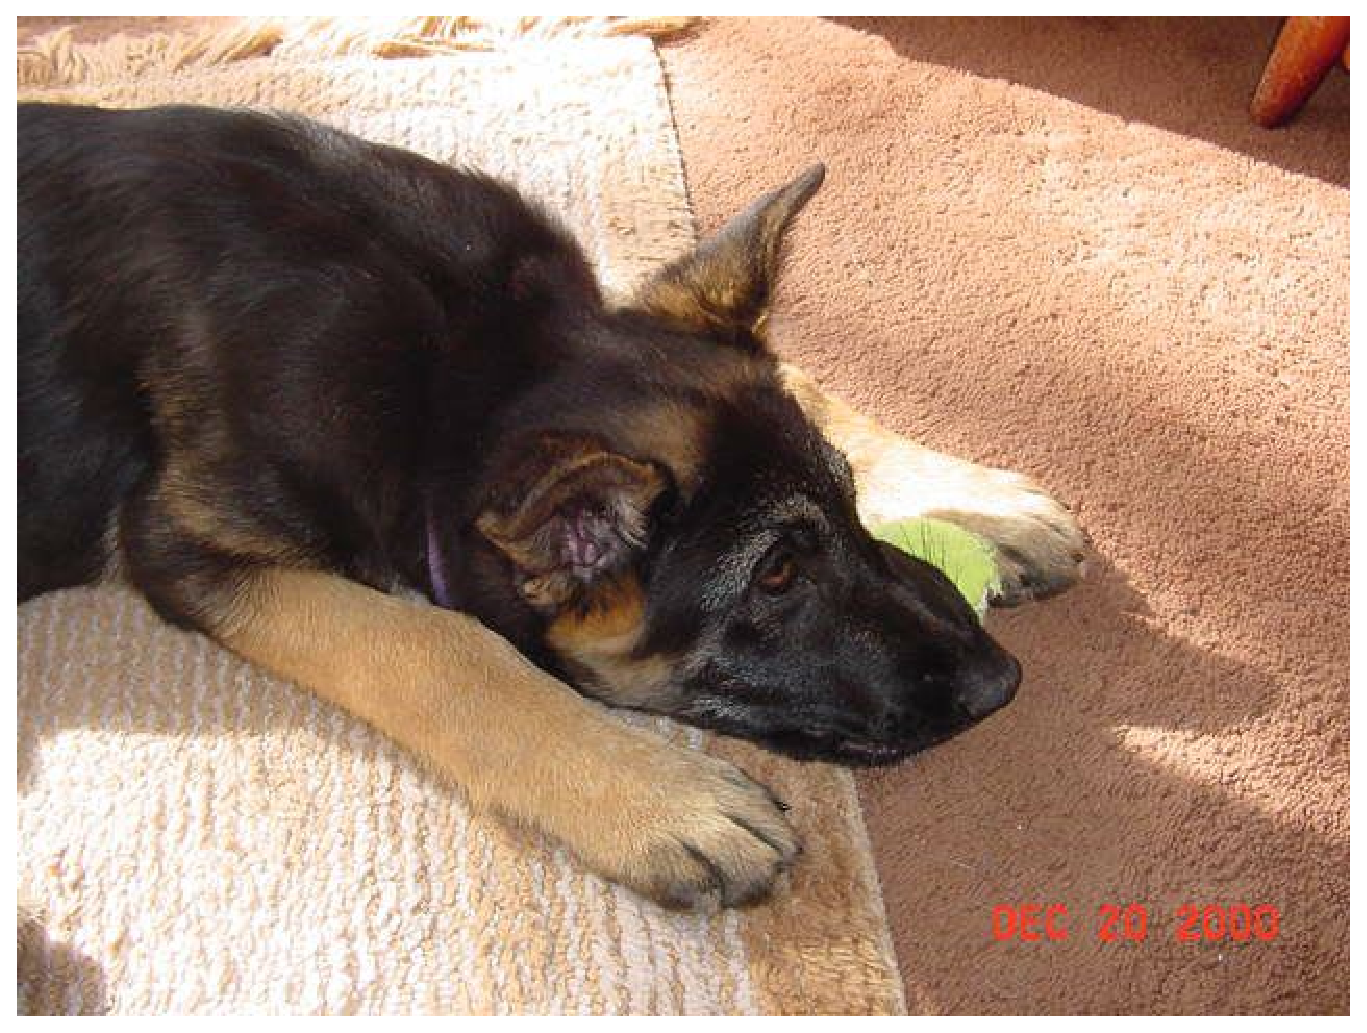
\psfig{file=pup-on-rug.eps,height=1.5in,width=2.0in}
\caption{An example of an imported eps file.}
\label{f:ex}
\end{center}
\end{figure}
\index{commands!environments!figure}%
You can see the commands that generated this
figure in the source file. Look for the line
\cn{begin\{figure\}[htb] \% Imported eps example. }

The command that imports the file is \cn{psfig}, and it also 
controls its size (\texttt{height} and \texttt{width}), and 
can rotate the figure (\texttt{angle}).

Figures can also be drawn by using \LaTeX{} commands. 
Figure \ref{f:circuit} is an example 
(taken from \cite{gms:tlc}).

\begin{figure}[htb] % Picture example.
\begin{center}
   \setlength{\unitlength}{4mm}
   \begin{picture}(12,10)(-2,0)
      \linethickness{0.4pt}
      \qbezier(2.00,6.00)(7.00,6.00)(9.00,3.00)
      \qbezier(2.00,0.00)(7.00,0.00)(9.00,3.00)
      \qbezier(2.00,6.00)(4.00,3.00)(2.00,0.00)
      \qbezier(1.00,6.00)(3.00,3.00)(1.00,0.00)
      \put(9.75,3.00){\circle{1.50}}
      \put(10.50,3.00){\line(1,0){1.50}}
      \put(0.00,5.00){\line(1,0){1.50}}
      \put(0.00,1.00){\line(1,0){1.50}}
   \end{picture}
\caption{An example of a picture}
\label{f:circuit}
\end{center}
\end{figure}
\index{picture}%

The commands that generated this
picture are in the source file following the line
\cn{begin\{figure\}[htb] \% Picture example.  }

The commands used have rather obvious meanings. In particular, 
the command \cn{qbezier} 
\index{commands!qbezier@\cn{qbezier}}%
draws a quadratic Bezier curve, 
defined by its two ending points, and a third point (whose 
coordinates are in the middle) that is used as control point. 
Figure \ref{f:qb} illustrates the effect of the control point:

%\begin{figure}[htb] % Bezier curves example.
\begin{figure}[h] % Bezier curves example.
\begin{center}
   \setlength{\unitlength}{.8mm}
   \begin{picture}(55,55)(-15,0)
      \linethickness{1pt}
      \qbezier(0,0)(-10,30)(50,30)
      \qbezier(0,0)(20,50)(50,30)
      \thinlines
      \put(0,0){\line(-1,3){10}}
      \put(50,30){\line(-1,0){60}}
      \put(0,0){\line(2,5){20}}
      \put(50,30){\line(-3,2){30}}
      \put(0,0){\circle*{1}}
      \put(0,-1){\makebox(0,0)[t]{$A_{0,0}$}}
      \put(-10,30){\circle*{1}}
      \put(-10,31){\makebox(0,0)[b]{$B_{10,30}$}}
      \put(50,30){\circle*{1}}
      \put(58,29){\makebox(0,0)[b]{$C_{50,30}$}}
      \put(20,50){\circle*{1}}
      \put(20,51){\makebox(0,0)[b]{$D_{20,50}$}}
   \end{picture}
\caption{Bezier curves}
\label{f:qb}
\end{center}
\end{figure}
\index{Bezier curves}%


This figure has been generated with the following commands:
\begin{verbatim}
\begin{figure}[htb] % Bezier curves example.
\begin{center}
   \setlength{\unitlength}{.8mm}
   \begin{picture}(55,55)(-15,0)
      \linethickness{1pt}
      \qbezier(0,0)(-10,30)(50,30)
      \qbezier(0,0)(20,50)(50,30)
      \thinlines
      \put(0,0){\line(-1,3){10}}
      \put(50,30){\line(-1,0){60}}
      \put(0,0){\line(2,5){20}}
      \put(50,30){\line(-3,2){30}}
      \put(0,0){\circle*{1}}
      \put(0,-1){\makebox(0,0)[t]{$A_{0,0}$}}
      \put(-10,30){\circle*{1}}
      \put(-10,31){\makebox(0,0)[b]{$B_{10,30}$}}
      \put(50,30){\circle*{1}}
      \put(58,29){\makebox(0,0)[b]{$C_{50,30}$}}
      \put(20,50){\circle*{1}}
      \put(20,51){\makebox(0,0)[b]{$D_{20,50}$}}
   \end{picture}
\caption{Bezier curves}
\label{f:qb}
\end{center}
\end{figure}
\end{verbatim}


\chapter{An Example of Mathematical Writing}
\index{An Example of Mathematical Writing%
@\emph{An Example of Mathematical Writing}}%

\section{Generalized Fatou's Lemma}
\index{Generalized Fatou's Lemma%
@\emph{Generalized Fatou's Lemma}}%

Here we show an application of the following lemma:

\begin{lem}[Generalized Fatou's Lemma] \label{l:fatou}

Let $A$ be a Dedekind ring and $F$ a rational series 
in $A[[X]]$, i.e., $F = p/q$ for some 
$p, q \in A[X]$. Then there exist two polynomials 
$P, Q \in A[X]$ such that $F = P/Q$, 
where $P$ and $Q$ are relatively prime and 
$Q(0) = 1$.

\end{lem}

\proof
See \cite{bertin:psn}, p.~15, theorem~1.3.
\endproof

\begin{thm} \label{l:req}
Let $\{c_n\}_{n=-\infty}^{\infty}$ a set of 
elements from $K$ such that $c_n \in k'$ for every 
$n \geq n_0$, and verifying the following recurrence 
relation of order M:
\begin{equation}
c_n\ =\ r_1\,c_{n-1} + r_2\,c_{n-2} + \dots + r_M\,c_{n-M}
\end{equation}
for every $n \in \mathbb Z$, where $r_1,r_2,\dots,r_M$ are in 
$K$, $r_M \neq 0$. 
Then:

\item{(i)} The coefficients $r_1,r_2,\dots,r_M$ are in 
$k'$, and for every $n \in \mathbb Z$, $c_n \in k'$.

\item{(ii)} If $c_n \in \mathcal O_{k',v}$ 
for every $n \geq n_0$, then the coefficients 
$r_1,r_2,\dots,r_M$ are all in 
$\mathcal O_{k',v}$.

\end{thm}


\proof 

\item{(i)} Let $C_n$ and $R$ be the matrices:

\begin{equation}
C_n\ =
\ \left(
\begin{array}{llll}
              c_n & c_{n+1} & \hdots & c_{n+M-1} \\
              c_{n+1} & c_{n+2} & \hdots  & c_{n+M} \\
              \vdots & \vdots & \ddots & \vdots \\
              c_{n+M-1} & c_{n+M} & \hdots & c_{n+2M-2}
\end{array}
\right)
\end{equation}
and
\begin{equation}
R\ =
\ \left(
\begin{array}{lllll}
              0 & 1 & 0 & \hdots & 0 \\
              0 & 0 & 1 & \hdots & 0 \\
             \vdots & \vdots & \vdots & \ddots & \vdots \\
              0 & 0 & 0 & \hdots & 1 \\
              r_M & r_{M-1} & r_{M-2} & \hdots & r_1 
\end{array}
\right)
\end{equation} 

We have that $C_{n+1} = R\,C_n$. Since the recurrence 
relation is of order M, $C_n$ is non singular. 
On the other hand, $R = C_{n+1}\,C_{n}^{-1}$. Since the 
elements of $C_n$ are in $k'$ for $n \geq n_0$, the entries 
of $R$, and those of $R^{-1}$, will be in $k'$. Since 
$C_{n-1} = R^{-1}\,C_n$, we get that the entries of 
$C_n$ will be in $k'$ also for $n < n_0$. 

\item{(ii)} For each $t \geq n_0$ define the formal 
power series 

\begin{equation}
F_t(X)\ =\ \sum_{n=0}^{\infty} c_{t+n}\,X^n
\end{equation}
which is in $\mathcal O_{k',v}[[X]]$. 
We have $F_t(X) = p_t(X)/q(X)$, 
where $p_t(X),q(X) \in k'[X]$ are the following:
\begin{equation}
p_t(X)\ =\ \sum_{j=0}^{M-1} \Bigl( c_{t+j} - 
                    \sum_{i=1}^{j} r_i\,c_{t+j-i} \Bigr)\,X^j
\end{equation}
\begin{equation}
q(X)\ =\ 1 - r_1\,X - r_2\,X^2 - \dots - r_M\,X^M
\end{equation}
This can be checked by multiplying $F_t(X)$ by $q_t(X)$ 
and using the recurrence relation, which gives 
$F_t(X)\,q(X) = p_t(X)$ (see \cite{poorten:sp}). 

Now we will prove that $p_t(X)$ and $q(X)$ are relatively 
prime. To do so, we will see that they cannot have any 
common root (in $\overline {k'}$). In fact, assume 
that $\alpha$ is a common root of $p_{t_0}(X)$ and $q(X)$ 
for some $t_0 \geq n_0$, i.e.: 
$p_{t_0}(\alpha) = q(\alpha) = 0$. 
Since $q(0)=1$, then $\alpha \neq 0$. Now we have:
\begin{equation}
X\,F_{t_0+1}(X) = F_{t_0}(X) - c_{t_0}
\end{equation}
so:
\begin{multline}
X\,p_{t_0+1}(X) = X\,q(X)\,F_{t_0+1}(X) \\
= q(X)\,(F_{t_0}(X) - c_{t_0}) = p_{t_0}(X) - c_{t_0}\,q(X)
\end{multline}
Hence $p_{t_0+1}(\alpha) = 0$, which means that $\alpha$ is 
also a root of $p_{t_0+1}(X)$. By induction we get that 
$p_t(\alpha) = 0$ for every $t \geq t_0$. Grouping the 
terms of $p_t(X)$ with respect to $c_t,c_{t+1},\dots,c_{t+M-1}$, 
we get:
\begin{equation}
p_t(X) = \sum_{j=0}^{M-1} a_j(X)\,c_{t+j}
\end{equation}
where 
\begin{equation}
a_j(X) = X^j\,\Bigl( 1 - \sum_{i=1}^{M-j-1} r_i\,X^i \Bigr)
\end{equation}
Note that $a_0(X),a_1(X),\dots,a_{M-1}(X)$ do not depend on t. 
On the other hand $p_t(\alpha)=0$ implies
\begin{equation}
\label{e:coldep}
\sum_{j=0}^{M-1} a_j(\alpha)\,c_{t+j} = 0
\end{equation}
for every $t \geq t_0$. Note that $a_{M-1}(\alpha)=\alpha^{M-1}
\neq 0$, so $a_0(\alpha),a_1(\alpha),\dots,a_{M-1}(\alpha)$ 
are not all zero, and (\ref{e:coldep}) means that the columns 
of the matrix $C_{t_0}$ are linearly dependent, so 
$\det C_{t_0}=0$, which contradicts the fact that $C_{t_0}$ 
is non singular. Hence, the hypothesis that $p_t(X)$ and 
$q(X)$ have a common root has to be false. This proves that 
$p_t(X)$ and $q(X)$ are relatively prime. 

By (generalized Fatou's) lemma~\ref{l:fatou}, 
and taking into account that 
$\mathcal O_{k',v}$ is a Dedekind ring, 
we get that there exist two relatively prime 
polynomials $P_t(X)$ and $Q_t(X)$ in 
$\mathcal O_{k',v}[X]$ such that 
$F_t(X) = P_t(X)/Q_t(X)$ and $Q_t(0)=1$. Hence: 
$p_t(X)\,Q_t(X) = q(X)\,P_t(X)$. By unique factorization 
of polynomials in $k'[X]$, there is a $u \in k'$ such that 
$P_t(X) = u\,p_t(X)$ and $Q_t(X) = u\,q_t(X)$. Since 
$Q_t(0)=q(0)=1$, we get that $u=1$, so 
$P_t(X) = p_t(X)$ and $Q_t(X) = q(X)$. 
Hence, the coefficients of $q(X)$ are in 
$\mathcal O_{k',v}$. 

\endproof


\section{Other Examples of Mathematical Writing}

\subsection{An Example of a Commutative Diagram}
\index{An Example of a Commutative Diagram%
@{An Example of a Commutative Diagram}}%

The following is an example of a commutative diagram.
\index{commutative diagram}%
It requires the \texttt{amscd} package.
\index{amscd package@{\texttt{amscd} package}}

\begin{equation*}
\newcommand{\End}{\operatorname{End}}
\begin{CD}
S^{{\mathcal{W}}_\Lambda}\otimes T   @>j>>   T\\
@VVV                                    @VV{\End P}V\\
(S\otimes T)/I                  @=      (Z\otimes T)/J
\end{CD}
\end{equation*}

That diagram has been made with the following commands:

\begin{verbatim}
\newcommand{\End}{\operatorname{End}}
\begin{CD}
S^{{\mathcal{W}}_\Lambda}\otimes T   @>j>>   T\\
@VVV                                    @VV{\End P}V\\
(S\otimes T)/I                  @=      (Z\otimes T)/J
\end{CD}
\end{verbatim}

\subsection{Using AMS Fonts}
\index{Using AMS Fonts@{Using AMS Fonts}}

To use AMS fonts it is necessary to choose from an assortment 
of \LaTeX{} packages. For instance the command 
\cn{usepackage\{amsfonts\}} calls in the \emph{amsfonts} package, 
which provides blackboard bold letters (e.g. $\mathbb{R}$) and 
some math symbols. A superset of that package is 
\emph{amssymb}. Other packages are \emph{eufrak} 
for Frankfurt letters (e.g. $\mathfrak{R}$)
and \emph{eucal} for Euler script 
(e.g. $\mathcal{R}$). 
Consult the \LaTeX{} documentation about this subject 
for additional information.

\appendices
\index{Appendices@\emph{Appendices}}%
\chapter{Lerma's Appendix}
\index{Appendix!Lerma's Appendix@\emph{Lerma's Appendix}}%
The source \LaTeX{} file for this document is no longer quoted in
its entirety in the output document. A \LaTeX{} file can 
include its own source by using the command
\cn{verbatiminput\{\cn{jobname}\}}.


%%%%%%%%%%%%%%%%%%%%%%%%%%%%%%%%%%%%%%%%%%
\chapter{My Appendix \#2}
\index{Appendix!My Appendix \#2@\emph{My Appendix \#2}}%
\section{The First Section}
This is the first section.
This is the second appendix.

\section{The Second Section}
This is the second section of the second appendix.

\subsection{The First Subsection of the Second Section}
This is the first subsection of the second section of the second appendix.

\subsection{The Second Subsection of the Second Section}
This is the second subsection of the second section of the second appendix.

\subsubsection{The First Subsubsection of the Second Subsection of
		the Second Section}
This is the first subsubsection of the second subsection of the
second section of the second appendix.

\subsubsection{The Second Subsubsection of the Second Subsection
		of the Second Section}
This is the second subsubsection of the second subsection of the
second section of the second appendix.

%%%%%%%%%%%%%%%%%%%%%%%%%%%%%%%%%%%%%%%%%%
\chapter{My Appendix \#3}
\index{Appendix!My Appendix \#3@\emph{My Appendix \#3}}%

\section{The First Section}
This is the first section.
This is the third appendix.

\section{The Second Section}
This is the second section of the third appendix.



\end{verbatim}
\index{commands!include@\cn{include}}%
Having the chapters in separate files makes the main .tex file simpler
and allows chapters to be easily re-ordered (just swap the order of the
include commands) or left (commented) out for draft copies.

Note: If you have only one appendix, in addition to using
\cn{appendix} instead of \cn{appendices}, you must leave out the
\cn{chapter} definition at the start of the appendix's text. Putting
it in will cause the insertion of an extra page with only the word
Appendix on it and will cause the appendix to be labeled Appendix 1,
both of which are poor form if there is only one appendix.

If you are writing a short dissertation 
\index{short dissertation}%
that does not require 
chapters, you need to use the command \cn{nochapters} 
\index{commands!nochapters@\cn{nochapters}}%
just before the first section:

\begin{verbatim}
\nochapters 

\section{...}     % First section.
    ... text ... 
\section{...}     % Second section.
    ... text ... 
        (...)
\end{verbatim}

Next comes the bibliography.
\index{bibliography}%
It can be made by hand like this:
\begin{verbatim}
\begin{thebibliography}{foo}
\bibitem ...   
\end{thebibliography}
\end{verbatim}
\index{commands!environments!thebibliography}%
Or it can also be generated with BiB\TeX{}, 
\index{BiBTeX@BiB\TeX{}}%
as explained in chapter \ref{c:bib}.

Finally the vita is produced like this:
\begin{verbatim}
\begin{vita}
     % Insert your brief biographical sketch here. 
     % Your permanent address and the name of the 
     % typist(s) are generated automatically.
\end{vita}

\end{verbatim}

\chapter{Making the Bibliography with BiB\TeX{}}\label{c:bib}
\index{Making the Bibliography with BiBTeX%
@\emph{Making the Bibliography with BiB\TeX{}}}%

BiB\TeX{} 
\index{BiBTeX@BiB\TeX{}}%
allows one to generate automatically the bibliography 
from a database of bibliographic 
items. You need to do the following:

\begin{enumerate}
\item Create the bibliographic database, 
\index{bibliographic database}%
which is a file whose name ends in \texttt{.bib}. 
\index{.bib@\texttt{.bib}}%
Let us call it \texttt{diss.bib}. Entries in this file are like this:
\begin{verbatim}
@BOOK{knuth:tb,
  author = "Donald K. Knuth",
  title = "The \TeXbook",
  publisher = "Addison-Wesley",
  year = "1984",
}
@TECHREPORT{poorten:sp,
  author = "Alf~J.~van der Poorten",
  title = "Some problems of recurrent interest",
  institution = "School of Mathematics and Physics,
                 Macquarie University",
  address = "North Ryde, Australia 2113",
  number = "81-0037",
  month = "August",
  year = "1981",
}
@ARTICLE{erdos:oap,
 author = "Paul Erd{\"o}s and Paul Turan",
 title = "On a problem in the theory of uniform 
          distribution, {I}", 
 journal = "Indag. Math.",
 volume = "10",
 year = "1948",
 pages = "370--378",
}
\end{verbatim}

\item Include a \cn{bibliographystyle} 
\index{commands!bibliographystyle@\cn{bibliographystyle}}%
command in your \LaTeX{} file, say 

\cn{bibliographystyle\{plain\}} 
and a \cn{bibliography} 
\index{commands!bibliography@\cn{bibliography}}%
command to load the bibliography, 
in this case \cn{bibliography\{diss\}}, at the point of your 
document where the bibliography should be inserted. 

The document at this point will look like this:
\begin{verbatim}
\bibliographystyle{plain}
\bibliography{diss}
\end{verbatim}

\item Run \LaTeX{} on your main file, say \texttt{foo.tex}: 
\texttt{latex foo}. This generates an auxiliary file 
\texttt{foo.aux} with a list of \cn{cite} 
\index{commands!cite@\cn{cite}}
references.

\item Run BiB\TeX{} on your file: \texttt{bibtex foo}. 
BiB\TeX{} reads the auxiliary file, looks up the 
bibliographic database (\texttt{diss.bib}), 
and writes a \texttt{.bbl} 
\index{.bbl@\texttt{.bbl}}%
file with the bibliographic information formated according to
the bibliographic style file (\texttt{.bst}, 
\index{.bst@\texttt{.bst}}%
say \texttt{plain.bst}) 
\index{plain.bst@\texttt{plain.bst}}%
specified.  Messages about resources used and error messages
are written to a \texttt{.blg} 
\index{.blg@\texttt{.blg}}%
file (in the case of this template, disstemplate.blg).

\item Run \LaTeX{} again: \texttt{latex foo}, which now 
reads the \texttt{.bbl} 
\index{.bbl@\texttt{.bbl}}%
reference file.

\item Run \LaTeX{} for a third time: \texttt{latex foo}, 
resolving all references.

\end{enumerate}

This includes all bibliographic items that have been cited 
in the document with a \cn{cite} 
\index{commands!cite@\cn{cite}}%
command. In order to include non cited items in the bibliography,
use the command \cn{nocite}. For example, \cn{nocite\{knuth:tb\}}
anywhere in the document (after \cn{begin\{document\}}) includes 
in the bibliography the item with label \texttt{knuth:tb}. 
In order to include \emph{all} items of the bibliographic 
database, use the command \cn{nocite\{*\}}.
\index{commands!nocite@\cn{nocite}}%

\chapter{Making Tables and Including Figures}
\index{Making Tables and Including Figures@\emph{Making Tables
	and Including Figures}}%

The \emph{tabular} 
\index{commands!environments!tabular}%
environment allows us to create complex 
tables and figures, and draw boundaries around and within it.
The following example illustrates this:

\begin{table}[h]
\begin{center}
\caption{An example of a table.}
\vskip 10pt
\begin{tabular}{|ll|l|ll|l|lll|}
\cline{1-2} \cline{4-5} \cline{7-9}
\multicolumn{2}{|c|} {\textsl{Gegenwart}} & &
\multicolumn{2}{|c|} {\textsl{Imperfekt}} & &
\multicolumn{3}{|c|} {\textsl{Perfekt}} \\
\cline{1-2} \cline{4-5} \cline{7-9}
ich & bin  & & ich & war   & & ich & bin  & gewesen \\
du  & bist & & du  & warst & & du  & bist & gewesen \\
er  &      & & er  &       & & er  &      &         \\
sie & ist  & & sie & wart  & & sie & ist  & gewesen \\
es  &      & & es  &       & & es  &      &         \\
\cline{1-2} \cline{4-5} \cline{7-9}
wir & sind & & wir & waren & & wir & sind & gewesen \\
ihr & seid & & ihr & wart  & & ihr & seid & gewesen \\
sie & sind & & sie & waren & & sie & sind & gewesen \\
\cline{1-2} \cline{4-5} \cline{7-9}
Sie & sind & & Sie & waren & & Sie & sind & gewesen \\
\cline{1-2} \cline{4-5} \cline{7-9}
\end{tabular} \\[10pt]
Note: The assistance of Herr Professor Lothar Frommhold \\
in generating this table of German declensions \\
is gratefully acknowledged.
\vskip -20pt
\end{center}
\end{table}
\index{commands!environments!table}%

This table was created with the following sequence 
of commands:
\begin{verbatim}
\begin{table}[h]
\begin{center}
\caption{An example of a table.}
\vskip 10pt
\begin{tabular}{|ll|l|ll|l|lll|}
\cline{1-2} \cline{4-5} \cline{7-9}
\multicolumn{2}{|c|} {\textsl{Gegenwart}} & &
\multicolumn{2}{|c|} {\textsl{Imperfekt}} & &
\multicolumn{3}{|c|} {\textsl{Perfekt}} \\
\cline{1-2} \cline{4-5} \cline{7-9}
ich & bin  & & ich & war   & & ich & bin  & gewesen \\
du  & bist & & du  & warst & & du  & bist & gewesen \\
er  &      & & er  &       & & er  &      &         \\
sie & ist  & & sie & wart  & & sie & ist  & gewesen \\
es  &      & & es  &       & & es  &      &         \\
\cline{1-2} \cline{4-5} \cline{7-9}
wir & sind & & wir & waren & & wir & sind & gewesen \\
ihr & seid & & ihr & wart  & & ihr & seid & gewesen \\
sie & sind & & sie & waren & & sie & sind & gewesen \\
\cline{1-2} \cline{4-5} \cline{7-9}
Sie & sind & & Sie & waren & & Sie & sind & gewesen \\
\cline{1-2} \cline{4-5} \cline{7-9}
\end{tabular} \\[10pt]
Note: The assistance of Herr Professor Lothar Frommhold \\
in generating this table of German declensions \\
is gratefully acknowledged.
\vskip -20pt
\end{center}
\end{table}
\index{commands!environments!table}%
\end{verbatim}

The argument \texttt{h} indicates the position for the 
table, in this case ``here if possible''. Other values
of this argument are:
\texttt{t} (top of the page),
\texttt{b} (bottom of the page),
\texttt{p} (on the page of floats) and 
\texttt{H} (HERE! - requires using the package float.sty.
Note: When this option is used, LaTeX ignores all of its formatting
rules and does what you say, putting the entire float exactly where
it is defined. Check your output to make sure it is what you want!
If you are having trouble with LaTeX wanting to put a figure that's
larger than roughly half-a-page, as well as all of the figures
following it, at the end of a chapter, try using the command
\cn{clearpage} immediately following the large figure --- and maybe
a \cn{newpage} later.)
It is possible to combine several arguments, such as
\texttt{ht} (``here if possible, otherwise on top of
the page''). The default is \texttt{tbp}.

Figure \ref{f:ex} is a typical example of inclusion of a 
figure contained in an encapsulated PostScript file. 
\index{PostScript}%
\index{encapsulated PostScript}%
In order to use it, it is necessary to include the 
command \cn{usepackage\{psfig\}} 
\index{psfig}%
at the beginning of the document.

\begin{figure}[htb] % Imported eps example.
\begin{center}
\ 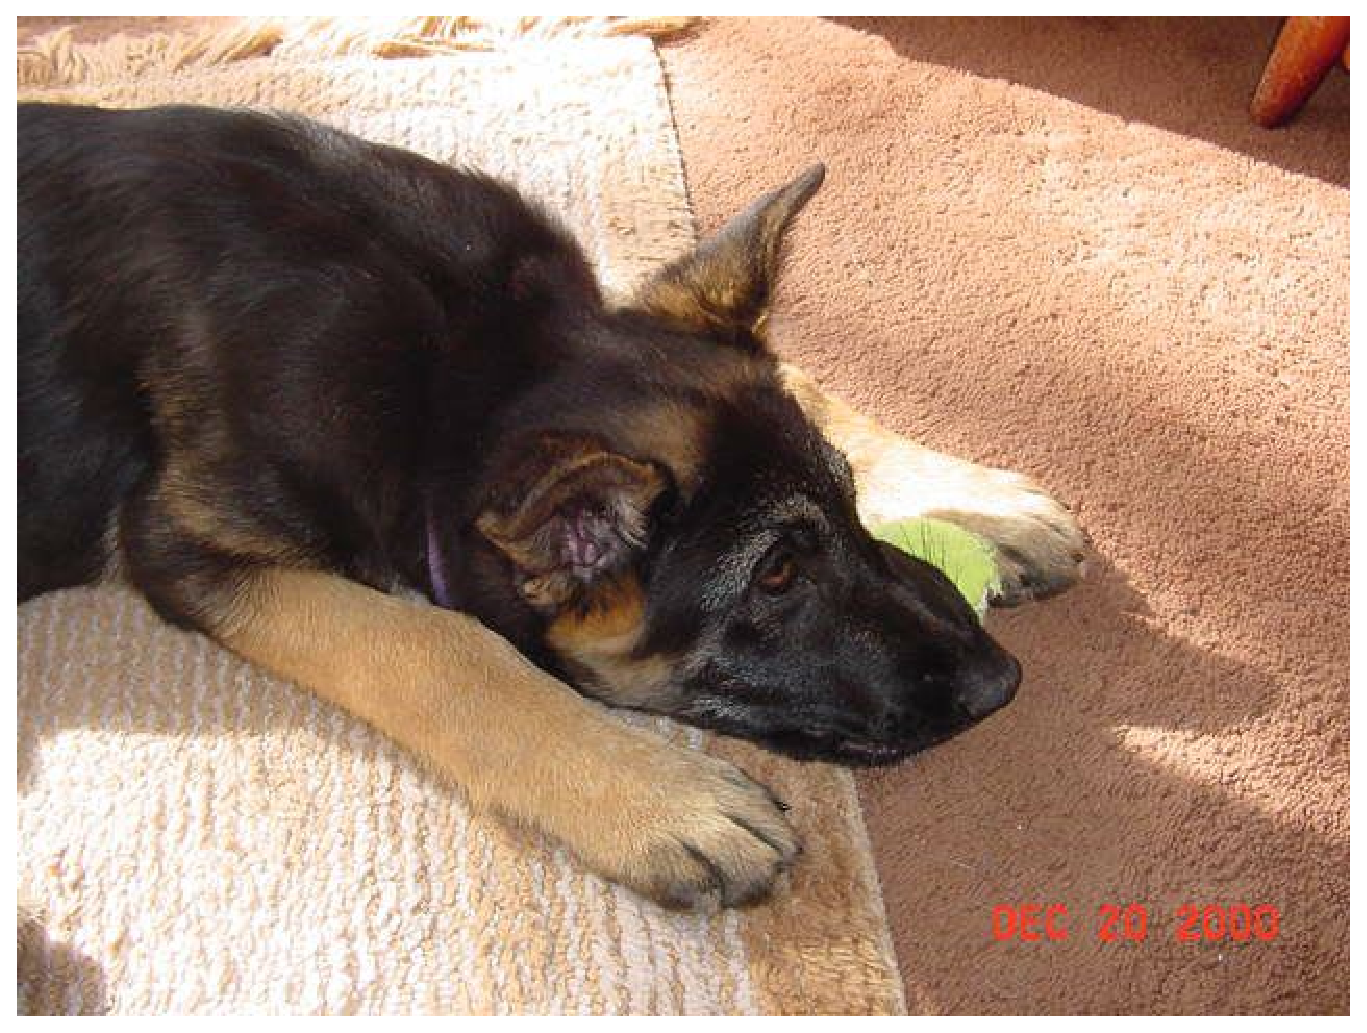
\psfig{file=pup-on-rug.eps,height=1.5in,width=2.0in}
\caption{An example of an imported eps file.}
\label{f:ex}
\end{center}
\end{figure}
\index{commands!environments!figure}%
You can see the commands that generated this
figure in the source file. Look for the line
\cn{begin\{figure\}[htb] \% Imported eps example. }

The command that imports the file is \cn{psfig}, and it also 
controls its size (\texttt{height} and \texttt{width}), and 
can rotate the figure (\texttt{angle}).

Figures can also be drawn by using \LaTeX{} commands. 
Figure \ref{f:circuit} is an example 
(taken from \cite{gms:tlc}).

\begin{figure}[htb] % Picture example.
\begin{center}
   \setlength{\unitlength}{4mm}
   \begin{picture}(12,10)(-2,0)
      \linethickness{0.4pt}
      \qbezier(2.00,6.00)(7.00,6.00)(9.00,3.00)
      \qbezier(2.00,0.00)(7.00,0.00)(9.00,3.00)
      \qbezier(2.00,6.00)(4.00,3.00)(2.00,0.00)
      \qbezier(1.00,6.00)(3.00,3.00)(1.00,0.00)
      \put(9.75,3.00){\circle{1.50}}
      \put(10.50,3.00){\line(1,0){1.50}}
      \put(0.00,5.00){\line(1,0){1.50}}
      \put(0.00,1.00){\line(1,0){1.50}}
   \end{picture}
\caption{An example of a picture}
\label{f:circuit}
\end{center}
\end{figure}
\index{picture}%

The commands that generated this
picture are in the source file following the line
\cn{begin\{figure\}[htb] \% Picture example.  }

The commands used have rather obvious meanings. In particular, 
the command \cn{qbezier} 
\index{commands!qbezier@\cn{qbezier}}%
draws a quadratic Bezier curve, 
defined by its two ending points, and a third point (whose 
coordinates are in the middle) that is used as control point. 
Figure \ref{f:qb} illustrates the effect of the control point:

%\begin{figure}[htb] % Bezier curves example.
\begin{figure}[h] % Bezier curves example.
\begin{center}
   \setlength{\unitlength}{.8mm}
   \begin{picture}(55,55)(-15,0)
      \linethickness{1pt}
      \qbezier(0,0)(-10,30)(50,30)
      \qbezier(0,0)(20,50)(50,30)
      \thinlines
      \put(0,0){\line(-1,3){10}}
      \put(50,30){\line(-1,0){60}}
      \put(0,0){\line(2,5){20}}
      \put(50,30){\line(-3,2){30}}
      \put(0,0){\circle*{1}}
      \put(0,-1){\makebox(0,0)[t]{$A_{0,0}$}}
      \put(-10,30){\circle*{1}}
      \put(-10,31){\makebox(0,0)[b]{$B_{10,30}$}}
      \put(50,30){\circle*{1}}
      \put(58,29){\makebox(0,0)[b]{$C_{50,30}$}}
      \put(20,50){\circle*{1}}
      \put(20,51){\makebox(0,0)[b]{$D_{20,50}$}}
   \end{picture}
\caption{Bezier curves}
\label{f:qb}
\end{center}
\end{figure}
\index{Bezier curves}%


This figure has been generated with the following commands:
\begin{verbatim}
\begin{figure}[htb] % Bezier curves example.
\begin{center}
   \setlength{\unitlength}{.8mm}
   \begin{picture}(55,55)(-15,0)
      \linethickness{1pt}
      \qbezier(0,0)(-10,30)(50,30)
      \qbezier(0,0)(20,50)(50,30)
      \thinlines
      \put(0,0){\line(-1,3){10}}
      \put(50,30){\line(-1,0){60}}
      \put(0,0){\line(2,5){20}}
      \put(50,30){\line(-3,2){30}}
      \put(0,0){\circle*{1}}
      \put(0,-1){\makebox(0,0)[t]{$A_{0,0}$}}
      \put(-10,30){\circle*{1}}
      \put(-10,31){\makebox(0,0)[b]{$B_{10,30}$}}
      \put(50,30){\circle*{1}}
      \put(58,29){\makebox(0,0)[b]{$C_{50,30}$}}
      \put(20,50){\circle*{1}}
      \put(20,51){\makebox(0,0)[b]{$D_{20,50}$}}
   \end{picture}
\caption{Bezier curves}
\label{f:qb}
\end{center}
\end{figure}
\end{verbatim}


\chapter{An Example of Mathematical Writing}
\index{An Example of Mathematical Writing%
@\emph{An Example of Mathematical Writing}}%

\section{Generalized Fatou's Lemma}
\index{Generalized Fatou's Lemma%
@\emph{Generalized Fatou's Lemma}}%

Here we show an application of the following lemma:

\begin{lem}[Generalized Fatou's Lemma] \label{l:fatou}

Let $A$ be a Dedekind ring and $F$ a rational series 
in $A[[X]]$, i.e., $F = p/q$ for some 
$p, q \in A[X]$. Then there exist two polynomials 
$P, Q \in A[X]$ such that $F = P/Q$, 
where $P$ and $Q$ are relatively prime and 
$Q(0) = 1$.

\end{lem}

\proof
See \cite{bertin:psn}, p.~15, theorem~1.3.
\endproof

\begin{thm} \label{l:req}
Let $\{c_n\}_{n=-\infty}^{\infty}$ a set of 
elements from $K$ such that $c_n \in k'$ for every 
$n \geq n_0$, and verifying the following recurrence 
relation of order M:
\begin{equation}
c_n\ =\ r_1\,c_{n-1} + r_2\,c_{n-2} + \dots + r_M\,c_{n-M}
\end{equation}
for every $n \in \mathbb Z$, where $r_1,r_2,\dots,r_M$ are in 
$K$, $r_M \neq 0$. 
Then:

\item{(i)} The coefficients $r_1,r_2,\dots,r_M$ are in 
$k'$, and for every $n \in \mathbb Z$, $c_n \in k'$.

\item{(ii)} If $c_n \in \mathcal O_{k',v}$ 
for every $n \geq n_0$, then the coefficients 
$r_1,r_2,\dots,r_M$ are all in 
$\mathcal O_{k',v}$.

\end{thm}


\proof 

\item{(i)} Let $C_n$ and $R$ be the matrices:

\begin{equation}
C_n\ =
\ \left(
\begin{array}{llll}
              c_n & c_{n+1} & \hdots & c_{n+M-1} \\
              c_{n+1} & c_{n+2} & \hdots  & c_{n+M} \\
              \vdots & \vdots & \ddots & \vdots \\
              c_{n+M-1} & c_{n+M} & \hdots & c_{n+2M-2}
\end{array}
\right)
\end{equation}
and
\begin{equation}
R\ =
\ \left(
\begin{array}{lllll}
              0 & 1 & 0 & \hdots & 0 \\
              0 & 0 & 1 & \hdots & 0 \\
             \vdots & \vdots & \vdots & \ddots & \vdots \\
              0 & 0 & 0 & \hdots & 1 \\
              r_M & r_{M-1} & r_{M-2} & \hdots & r_1 
\end{array}
\right)
\end{equation} 

We have that $C_{n+1} = R\,C_n$. Since the recurrence 
relation is of order M, $C_n$ is non singular. 
On the other hand, $R = C_{n+1}\,C_{n}^{-1}$. Since the 
elements of $C_n$ are in $k'$ for $n \geq n_0$, the entries 
of $R$, and those of $R^{-1}$, will be in $k'$. Since 
$C_{n-1} = R^{-1}\,C_n$, we get that the entries of 
$C_n$ will be in $k'$ also for $n < n_0$. 

\item{(ii)} For each $t \geq n_0$ define the formal 
power series 

\begin{equation}
F_t(X)\ =\ \sum_{n=0}^{\infty} c_{t+n}\,X^n
\end{equation}
which is in $\mathcal O_{k',v}[[X]]$. 
We have $F_t(X) = p_t(X)/q(X)$, 
where $p_t(X),q(X) \in k'[X]$ are the following:
\begin{equation}
p_t(X)\ =\ \sum_{j=0}^{M-1} \Bigl( c_{t+j} - 
                    \sum_{i=1}^{j} r_i\,c_{t+j-i} \Bigr)\,X^j
\end{equation}
\begin{equation}
q(X)\ =\ 1 - r_1\,X - r_2\,X^2 - \dots - r_M\,X^M
\end{equation}
This can be checked by multiplying $F_t(X)$ by $q_t(X)$ 
and using the recurrence relation, which gives 
$F_t(X)\,q(X) = p_t(X)$ (see \cite{poorten:sp}). 

Now we will prove that $p_t(X)$ and $q(X)$ are relatively 
prime. To do so, we will see that they cannot have any 
common root (in $\overline {k'}$). In fact, assume 
that $\alpha$ is a common root of $p_{t_0}(X)$ and $q(X)$ 
for some $t_0 \geq n_0$, i.e.: 
$p_{t_0}(\alpha) = q(\alpha) = 0$. 
Since $q(0)=1$, then $\alpha \neq 0$. Now we have:
\begin{equation}
X\,F_{t_0+1}(X) = F_{t_0}(X) - c_{t_0}
\end{equation}
so:
\begin{multline}
X\,p_{t_0+1}(X) = X\,q(X)\,F_{t_0+1}(X) \\
= q(X)\,(F_{t_0}(X) - c_{t_0}) = p_{t_0}(X) - c_{t_0}\,q(X)
\end{multline}
Hence $p_{t_0+1}(\alpha) = 0$, which means that $\alpha$ is 
also a root of $p_{t_0+1}(X)$. By induction we get that 
$p_t(\alpha) = 0$ for every $t \geq t_0$. Grouping the 
terms of $p_t(X)$ with respect to $c_t,c_{t+1},\dots,c_{t+M-1}$, 
we get:
\begin{equation}
p_t(X) = \sum_{j=0}^{M-1} a_j(X)\,c_{t+j}
\end{equation}
where 
\begin{equation}
a_j(X) = X^j\,\Bigl( 1 - \sum_{i=1}^{M-j-1} r_i\,X^i \Bigr)
\end{equation}
Note that $a_0(X),a_1(X),\dots,a_{M-1}(X)$ do not depend on t. 
On the other hand $p_t(\alpha)=0$ implies
\begin{equation}
\label{e:coldep}
\sum_{j=0}^{M-1} a_j(\alpha)\,c_{t+j} = 0
\end{equation}
for every $t \geq t_0$. Note that $a_{M-1}(\alpha)=\alpha^{M-1}
\neq 0$, so $a_0(\alpha),a_1(\alpha),\dots,a_{M-1}(\alpha)$ 
are not all zero, and (\ref{e:coldep}) means that the columns 
of the matrix $C_{t_0}$ are linearly dependent, so 
$\det C_{t_0}=0$, which contradicts the fact that $C_{t_0}$ 
is non singular. Hence, the hypothesis that $p_t(X)$ and 
$q(X)$ have a common root has to be false. This proves that 
$p_t(X)$ and $q(X)$ are relatively prime. 

By (generalized Fatou's) lemma~\ref{l:fatou}, 
and taking into account that 
$\mathcal O_{k',v}$ is a Dedekind ring, 
we get that there exist two relatively prime 
polynomials $P_t(X)$ and $Q_t(X)$ in 
$\mathcal O_{k',v}[X]$ such that 
$F_t(X) = P_t(X)/Q_t(X)$ and $Q_t(0)=1$. Hence: 
$p_t(X)\,Q_t(X) = q(X)\,P_t(X)$. By unique factorization 
of polynomials in $k'[X]$, there is a $u \in k'$ such that 
$P_t(X) = u\,p_t(X)$ and $Q_t(X) = u\,q_t(X)$. Since 
$Q_t(0)=q(0)=1$, we get that $u=1$, so 
$P_t(X) = p_t(X)$ and $Q_t(X) = q(X)$. 
Hence, the coefficients of $q(X)$ are in 
$\mathcal O_{k',v}$. 

\endproof


\section{Other Examples of Mathematical Writing}

\subsection{An Example of a Commutative Diagram}
\index{An Example of a Commutative Diagram%
@{An Example of a Commutative Diagram}}%

The following is an example of a commutative diagram.
\index{commutative diagram}%
It requires the \texttt{amscd} package.
\index{amscd package@{\texttt{amscd} package}}

\begin{equation*}
\newcommand{\End}{\operatorname{End}}
\begin{CD}
S^{{\mathcal{W}}_\Lambda}\otimes T   @>j>>   T\\
@VVV                                    @VV{\End P}V\\
(S\otimes T)/I                  @=      (Z\otimes T)/J
\end{CD}
\end{equation*}

That diagram has been made with the following commands:

\begin{verbatim}
\newcommand{\End}{\operatorname{End}}
\begin{CD}
S^{{\mathcal{W}}_\Lambda}\otimes T   @>j>>   T\\
@VVV                                    @VV{\End P}V\\
(S\otimes T)/I                  @=      (Z\otimes T)/J
\end{CD}
\end{verbatim}

\subsection{Using AMS Fonts}
\index{Using AMS Fonts@{Using AMS Fonts}}

To use AMS fonts it is necessary to choose from an assortment 
of \LaTeX{} packages. For instance the command 
\cn{usepackage\{amsfonts\}} calls in the \emph{amsfonts} package, 
which provides blackboard bold letters (e.g. $\mathbb{R}$) and 
some math symbols. A superset of that package is 
\emph{amssymb}. Other packages are \emph{eufrak} 
for Frankfurt letters (e.g. $\mathfrak{R}$)
and \emph{eucal} for Euler script 
(e.g. $\mathcal{R}$). 
Consult the \LaTeX{} documentation about this subject 
for additional information.

\appendices
\index{Appendices@\emph{Appendices}}%
\chapter{Lerma's Appendix}
\index{Appendix!Lerma's Appendix@\emph{Lerma's Appendix}}%
The source \LaTeX{} file for this document is no longer quoted in
its entirety in the output document. A \LaTeX{} file can 
include its own source by using the command
\cn{verbatiminput\{\cn{jobname}\}}.


%%%%%%%%%%%%%%%%%%%%%%%%%%%%%%%%%%%%%%%%%%
\chapter{My Appendix \#2}
\index{Appendix!My Appendix \#2@\emph{My Appendix \#2}}%
\section{The First Section}
This is the first section.
This is the second appendix.

\section{The Second Section}
This is the second section of the second appendix.

\subsection{The First Subsection of the Second Section}
This is the first subsection of the second section of the second appendix.

\subsection{The Second Subsection of the Second Section}
This is the second subsection of the second section of the second appendix.

\subsubsection{The First Subsubsection of the Second Subsection of
		the Second Section}
This is the first subsubsection of the second subsection of the
second section of the second appendix.

\subsubsection{The Second Subsubsection of the Second Subsection
		of the Second Section}
This is the second subsubsection of the second subsection of the
second section of the second appendix.

%%%%%%%%%%%%%%%%%%%%%%%%%%%%%%%%%%%%%%%%%%
\chapter{My Appendix \#3}
\index{Appendix!My Appendix \#3@\emph{My Appendix \#3}}%

\section{The First Section}
This is the first section.
This is the third appendix.

\section{The Second Section}
This is the second section of the third appendix.



\end{verbatim}
\index{commands!include@\cn{include}}%
Having the chapters in separate files makes the main .tex file simpler
and allows chapters to be easily re-ordered (just swap the order of the
include commands) or left (commented) out for draft copies.

Note: If you have only one appendix, in addition to using
\cn{appendix} instead of \cn{appendices}, you must leave out the
\cn{chapter} definition at the start of the appendix's text. Putting
it in will cause the insertion of an extra page with only the word
Appendix on it and will cause the appendix to be labeled Appendix 1,
both of which are poor form if there is only one appendix.

If you are writing a short dissertation 
\index{short dissertation}%
that does not require 
chapters, you need to use the command \cn{nochapters} 
\index{commands!nochapters@\cn{nochapters}}%
just before the first section:

\begin{verbatim}
\nochapters 

\section{...}     % First section.
    ... text ... 
\section{...}     % Second section.
    ... text ... 
        (...)
\end{verbatim}

Next comes the bibliography.
\index{bibliography}%
It can be made by hand like this:
\begin{verbatim}
\begin{thebibliography}{foo}
\bibitem ...   
\end{thebibliography}
\end{verbatim}
\index{commands!environments!thebibliography}%
Or it can also be generated with BiB\TeX{}, 
\index{BiBTeX@BiB\TeX{}}%
as explained in chapter \ref{c:bib}.

Finally the vita is produced like this:
\begin{verbatim}
\begin{vita}
     % Insert your brief biographical sketch here. 
     % Your permanent address and the name of the 
     % typist(s) are generated automatically.
\end{vita}

\end{verbatim}


\chapter{Making the Bibliography with BiB\TeX{}}\label{c:bib}
\index{Making the Bibliography with BiBTeX%
@\emph{Making the Bibliography with BiB\TeX{}}}%

BiB\TeX{} 
\index{BiBTeX@BiB\TeX{}}%
allows one to generate automatically the bibliography 
from a database of bibliographic 
items. You need to do the following:

\begin{enumerate}
\item Create the bibliographic database, 
\index{bibliographic database}%
which is a file whose name ends in \texttt{.bib}. 
\index{.bib@\texttt{.bib}}%
Let us call it \texttt{diss.bib}. Entries in this file are like this:
\begin{verbatim}
@BOOK{knuth:tb,
  author = "Donald K. Knuth",
  title = "The \TeXbook",
  publisher = "Addison-Wesley",
  year = "1984",
}
@TECHREPORT{poorten:sp,
  author = "Alf~J.~van der Poorten",
  title = "Some problems of recurrent interest",
  institution = "School of Mathematics and Physics,
                 Macquarie University",
  address = "North Ryde, Australia 2113",
  number = "81-0037",
  month = "August",
  year = "1981",
}
@ARTICLE{erdos:oap,
 author = "Paul Erd{\"o}s and Paul Turan",
 title = "On a problem in the theory of uniform 
          distribution, {I}", 
 journal = "Indag. Math.",
 volume = "10",
 year = "1948",
 pages = "370--378",
}
\end{verbatim}

\item Include a \cn{bibliographystyle} 
\index{commands!bibliographystyle@\cn{bibliographystyle}}%
command in your \LaTeX{} file, say 

\cn{bibliographystyle\{plain\}} 
and a \cn{bibliography} 
\index{commands!bibliography@\cn{bibliography}}%
command to load the bibliography, 
in this case \cn{bibliography\{diss\}}, at the point of your 
document where the bibliography should be inserted. 

The document at this point will look like this:
\begin{verbatim}
\bibliographystyle{plain}
\bibliography{diss}
\end{verbatim}

\item Run \LaTeX{} on your main file, say \texttt{foo.tex}: 
\texttt{latex foo}. This generates an auxiliary file 
\texttt{foo.aux} with a list of \cn{cite} 
\index{commands!cite@\cn{cite}}
references.

\item Run BiB\TeX{} on your file: \texttt{bibtex foo}. 
BiB\TeX{} reads the auxiliary file, looks up the 
bibliographic database (\texttt{diss.bib}), 
and writes a \texttt{.bbl} 
\index{.bbl@\texttt{.bbl}}%
file with the bibliographic information formated according to
the bibliographic style file (\texttt{.bst}, 
\index{.bst@\texttt{.bst}}%
say \texttt{plain.bst}) 
\index{plain.bst@\texttt{plain.bst}}%
specified.  Messages about resources used and error messages
are written to a \texttt{.blg} 
\index{.blg@\texttt{.blg}}%
file (in the case of this template, disstemplate.blg).

\item Run \LaTeX{} again: \texttt{latex foo}, which now 
reads the \texttt{.bbl} 
\index{.bbl@\texttt{.bbl}}%
reference file.

\item Run \LaTeX{} for a third time: \texttt{latex foo}, 
resolving all references.

\end{enumerate}

This includes all bibliographic items that have been cited 
in the document with a \cn{cite} 
\index{commands!cite@\cn{cite}}%
command. In order to include non cited items in the bibliography,
use the command \cn{nocite}. For example, \cn{nocite\{knuth:tb\}}
anywhere in the document (after \cn{begin\{document\}}) includes 
in the bibliography the item with label \texttt{knuth:tb}. 
In order to include \emph{all} items of the bibliographic 
database, use the command \cn{nocite\{*\}}.
\index{commands!nocite@\cn{nocite}}%


\chapter{Making Tables and Including Figures}
\index{Making Tables and Including Figures@\emph{Making Tables
	and Including Figures}}%

The \emph{tabular} 
\index{commands!environments!tabular}%
environment allows us to create complex 
tables and figures, and draw boundaries around and within it.
The following example illustrates this:

\begin{table}[h]
\begin{center}
\caption{An example of a table.}
\vskip 10pt
\begin{tabular}{|ll|l|ll|l|lll|}
\cline{1-2} \cline{4-5} \cline{7-9}
\multicolumn{2}{|c|} {\textsl{Gegenwart}} & &
\multicolumn{2}{|c|} {\textsl{Imperfekt}} & &
\multicolumn{3}{|c|} {\textsl{Perfekt}} \\
\cline{1-2} \cline{4-5} \cline{7-9}
ich & bin  & & ich & war   & & ich & bin  & gewesen \\
du  & bist & & du  & warst & & du  & bist & gewesen \\
er  &      & & er  &       & & er  &      &         \\
sie & ist  & & sie & wart  & & sie & ist  & gewesen \\
es  &      & & es  &       & & es  &      &         \\
\cline{1-2} \cline{4-5} \cline{7-9}
wir & sind & & wir & waren & & wir & sind & gewesen \\
ihr & seid & & ihr & wart  & & ihr & seid & gewesen \\
sie & sind & & sie & waren & & sie & sind & gewesen \\
\cline{1-2} \cline{4-5} \cline{7-9}
Sie & sind & & Sie & waren & & Sie & sind & gewesen \\
\cline{1-2} \cline{4-5} \cline{7-9}
\end{tabular} \\[10pt]
Note: The assistance of Herr Professor Lothar Frommhold \\
in generating this table of German declensions \\
is gratefully acknowledged.
\vskip -20pt
\end{center}
\end{table}
\index{commands!environments!table}%

This table was created with the following sequence 
of commands:
\begin{verbatim}
\begin{table}[h]
\begin{center}
\caption{An example of a table.}
\vskip 10pt
\begin{tabular}{|ll|l|ll|l|lll|}
\cline{1-2} \cline{4-5} \cline{7-9}
\multicolumn{2}{|c|} {\textsl{Gegenwart}} & &
\multicolumn{2}{|c|} {\textsl{Imperfekt}} & &
\multicolumn{3}{|c|} {\textsl{Perfekt}} \\
\cline{1-2} \cline{4-5} \cline{7-9}
ich & bin  & & ich & war   & & ich & bin  & gewesen \\
du  & bist & & du  & warst & & du  & bist & gewesen \\
er  &      & & er  &       & & er  &      &         \\
sie & ist  & & sie & wart  & & sie & ist  & gewesen \\
es  &      & & es  &       & & es  &      &         \\
\cline{1-2} \cline{4-5} \cline{7-9}
wir & sind & & wir & waren & & wir & sind & gewesen \\
ihr & seid & & ihr & wart  & & ihr & seid & gewesen \\
sie & sind & & sie & waren & & sie & sind & gewesen \\
\cline{1-2} \cline{4-5} \cline{7-9}
Sie & sind & & Sie & waren & & Sie & sind & gewesen \\
\cline{1-2} \cline{4-5} \cline{7-9}
\end{tabular} \\[10pt]
Note: The assistance of Herr Professor Lothar Frommhold \\
in generating this table of German declensions \\
is gratefully acknowledged.
\vskip -20pt
\end{center}
\end{table}
\index{commands!environments!table}%
\end{verbatim}

The argument \texttt{h} indicates the position for the 
table, in this case ``here if possible''. Other values
of this argument are:
\texttt{t} (top of the page),
\texttt{b} (bottom of the page),
\texttt{p} (on the page of floats) and 
\texttt{H} (HERE! - requires using the package float.sty.
Note: When this option is used, LaTeX ignores all of its formatting
rules and does what you say, putting the entire float exactly where
it is defined. Check your output to make sure it is what you want!
If you are having trouble with LaTeX wanting to put a figure that's
larger than roughly half-a-page, as well as all of the figures
following it, at the end of a chapter, try using the command
\cn{clearpage} immediately following the large figure --- and maybe
a \cn{newpage} later.)
It is possible to combine several arguments, such as
\texttt{ht} (``here if possible, otherwise on top of
the page''). The default is \texttt{tbp}.

Figure \ref{f:ex} is a typical example of inclusion of a 
figure contained in an encapsulated PostScript file. 
\index{PostScript}%
\index{encapsulated PostScript}%
In order to use it, it is necessary to include the 
command \cn{usepackage\{psfig\}} 
\index{psfig}%
at the beginning of the document.

\begin{figure}[htb] % Imported eps example.
\begin{center}
\ 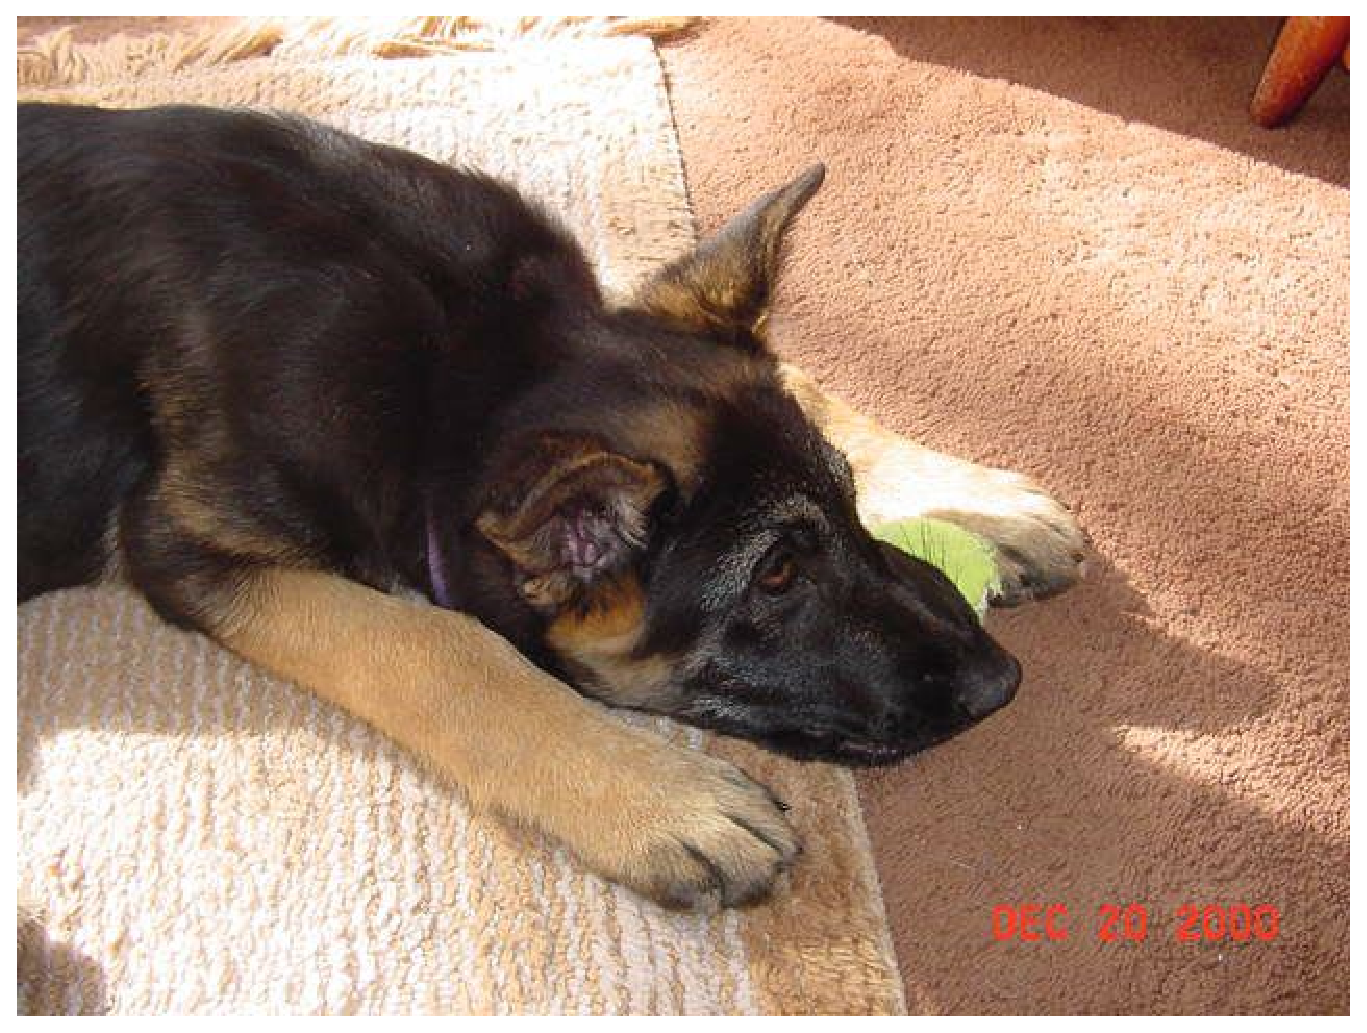
\psfig{file=pup-on-rug.eps,height=1.5in,width=2.0in}
\caption{An example of an imported eps file.}
\label{f:ex}
\end{center}
\end{figure}
\index{commands!environments!figure}%
You can see the commands that generated this
figure in the source file. Look for the line
\cn{begin\{figure\}[htb] \% Imported eps example. }

The command that imports the file is \cn{psfig}, and it also 
controls its size (\texttt{height} and \texttt{width}), and 
can rotate the figure (\texttt{angle}).

Figures can also be drawn by using \LaTeX{} commands. 
Figure \ref{f:circuit} is an example 
(taken from \cite{gms:tlc}).

\begin{figure}[htb] % Picture example.
\begin{center}
   \setlength{\unitlength}{4mm}
   \begin{picture}(12,10)(-2,0)
      \linethickness{0.4pt}
      \qbezier(2.00,6.00)(7.00,6.00)(9.00,3.00)
      \qbezier(2.00,0.00)(7.00,0.00)(9.00,3.00)
      \qbezier(2.00,6.00)(4.00,3.00)(2.00,0.00)
      \qbezier(1.00,6.00)(3.00,3.00)(1.00,0.00)
      \put(9.75,3.00){\circle{1.50}}
      \put(10.50,3.00){\line(1,0){1.50}}
      \put(0.00,5.00){\line(1,0){1.50}}
      \put(0.00,1.00){\line(1,0){1.50}}
   \end{picture}
\caption{An example of a picture}
\label{f:circuit}
\end{center}
\end{figure}
\index{picture}%

The commands that generated this
picture are in the source file following the line
\cn{begin\{figure\}[htb] \% Picture example.  }

The commands used have rather obvious meanings. In particular, 
the command \cn{qbezier} 
\index{commands!qbezier@\cn{qbezier}}%
draws a quadratic Bezier curve, 
defined by its two ending points, and a third point (whose 
coordinates are in the middle) that is used as control point. 
Figure \ref{f:qb} illustrates the effect of the control point:

%\begin{figure}[htb] % Bezier curves example.
\begin{figure}[h] % Bezier curves example.
\begin{center}
   \setlength{\unitlength}{.8mm}
   \begin{picture}(55,55)(-15,0)
      \linethickness{1pt}
      \qbezier(0,0)(-10,30)(50,30)
      \qbezier(0,0)(20,50)(50,30)
      \thinlines
      \put(0,0){\line(-1,3){10}}
      \put(50,30){\line(-1,0){60}}
      \put(0,0){\line(2,5){20}}
      \put(50,30){\line(-3,2){30}}
      \put(0,0){\circle*{1}}
      \put(0,-1){\makebox(0,0)[t]{$A_{0,0}$}}
      \put(-10,30){\circle*{1}}
      \put(-10,31){\makebox(0,0)[b]{$B_{10,30}$}}
      \put(50,30){\circle*{1}}
      \put(58,29){\makebox(0,0)[b]{$C_{50,30}$}}
      \put(20,50){\circle*{1}}
      \put(20,51){\makebox(0,0)[b]{$D_{20,50}$}}
   \end{picture}
\caption{Bezier curves}
\label{f:qb}
\end{center}
\end{figure}
\index{Bezier curves}%


This figure has been generated with the following commands:
\begin{verbatim}
\begin{figure}[htb] % Bezier curves example.
\begin{center}
   \setlength{\unitlength}{.8mm}
   \begin{picture}(55,55)(-15,0)
      \linethickness{1pt}
      \qbezier(0,0)(-10,30)(50,30)
      \qbezier(0,0)(20,50)(50,30)
      \thinlines
      \put(0,0){\line(-1,3){10}}
      \put(50,30){\line(-1,0){60}}
      \put(0,0){\line(2,5){20}}
      \put(50,30){\line(-3,2){30}}
      \put(0,0){\circle*{1}}
      \put(0,-1){\makebox(0,0)[t]{$A_{0,0}$}}
      \put(-10,30){\circle*{1}}
      \put(-10,31){\makebox(0,0)[b]{$B_{10,30}$}}
      \put(50,30){\circle*{1}}
      \put(58,29){\makebox(0,0)[b]{$C_{50,30}$}}
      \put(20,50){\circle*{1}}
      \put(20,51){\makebox(0,0)[b]{$D_{20,50}$}}
   \end{picture}
\caption{Bezier curves}
\label{f:qb}
\end{center}
\end{figure}
\end{verbatim}



\chapter{An Example of Mathematical Writing}
\index{An Example of Mathematical Writing%
@\emph{An Example of Mathematical Writing}}%

\section{Generalized Fatou's Lemma}
\index{Generalized Fatou's Lemma%
@\emph{Generalized Fatou's Lemma}}%

Here we show an application of the following lemma:

\begin{lem}[Generalized Fatou's Lemma] \label{l:fatou}

Let $A$ be a Dedekind ring and $F$ a rational series 
in $A[[X]]$, i.e., $F = p/q$ for some 
$p, q \in A[X]$. Then there exist two polynomials 
$P, Q \in A[X]$ such that $F = P/Q$, 
where $P$ and $Q$ are relatively prime and 
$Q(0) = 1$.

\end{lem}

\proof
See \cite{bertin:psn}, p.~15, theorem~1.3.
\endproof

\begin{thm} \label{l:req}
Let $\{c_n\}_{n=-\infty}^{\infty}$ a set of 
elements from $K$ such that $c_n \in k'$ for every 
$n \geq n_0$, and verifying the following recurrence 
relation of order M:
\begin{equation}
c_n\ =\ r_1\,c_{n-1} + r_2\,c_{n-2} + \dots + r_M\,c_{n-M}
\end{equation}
for every $n \in \mathbb Z$, where $r_1,r_2,\dots,r_M$ are in 
$K$, $r_M \neq 0$. 
Then:

\item{(i)} The coefficients $r_1,r_2,\dots,r_M$ are in 
$k'$, and for every $n \in \mathbb Z$, $c_n \in k'$.

\item{(ii)} If $c_n \in \mathcal O_{k',v}$ 
for every $n \geq n_0$, then the coefficients 
$r_1,r_2,\dots,r_M$ are all in 
$\mathcal O_{k',v}$.

\end{thm}


\proof 

\item{(i)} Let $C_n$ and $R$ be the matrices:

\begin{equation}
C_n\ =
\ \left(
\begin{array}{llll}
              c_n & c_{n+1} & \hdots & c_{n+M-1} \\
              c_{n+1} & c_{n+2} & \hdots  & c_{n+M} \\
              \vdots & \vdots & \ddots & \vdots \\
              c_{n+M-1} & c_{n+M} & \hdots & c_{n+2M-2}
\end{array}
\right)
\end{equation}
and
\begin{equation}
R\ =
\ \left(
\begin{array}{lllll}
              0 & 1 & 0 & \hdots & 0 \\
              0 & 0 & 1 & \hdots & 0 \\
             \vdots & \vdots & \vdots & \ddots & \vdots \\
              0 & 0 & 0 & \hdots & 1 \\
              r_M & r_{M-1} & r_{M-2} & \hdots & r_1 
\end{array}
\right)
\end{equation} 

We have that $C_{n+1} = R\,C_n$. Since the recurrence 
relation is of order M, $C_n$ is non singular. 
On the other hand, $R = C_{n+1}\,C_{n}^{-1}$. Since the 
elements of $C_n$ are in $k'$ for $n \geq n_0$, the entries 
of $R$, and those of $R^{-1}$, will be in $k'$. Since 
$C_{n-1} = R^{-1}\,C_n$, we get that the entries of 
$C_n$ will be in $k'$ also for $n < n_0$. 

\item{(ii)} For each $t \geq n_0$ define the formal 
power series 

\begin{equation}
F_t(X)\ =\ \sum_{n=0}^{\infty} c_{t+n}\,X^n
\end{equation}
which is in $\mathcal O_{k',v}[[X]]$. 
We have $F_t(X) = p_t(X)/q(X)$, 
where $p_t(X),q(X) \in k'[X]$ are the following:
\begin{equation}
p_t(X)\ =\ \sum_{j=0}^{M-1} \Bigl( c_{t+j} - 
                    \sum_{i=1}^{j} r_i\,c_{t+j-i} \Bigr)\,X^j
\end{equation}
\begin{equation}
q(X)\ =\ 1 - r_1\,X - r_2\,X^2 - \dots - r_M\,X^M
\end{equation}
This can be checked by multiplying $F_t(X)$ by $q_t(X)$ 
and using the recurrence relation, which gives 
$F_t(X)\,q(X) = p_t(X)$ (see \cite{poorten:sp}). 

Now we will prove that $p_t(X)$ and $q(X)$ are relatively 
prime. To do so, we will see that they cannot have any 
common root (in $\overline {k'}$). In fact, assume 
that $\alpha$ is a common root of $p_{t_0}(X)$ and $q(X)$ 
for some $t_0 \geq n_0$, i.e.: 
$p_{t_0}(\alpha) = q(\alpha) = 0$. 
Since $q(0)=1$, then $\alpha \neq 0$. Now we have:
\begin{equation}
X\,F_{t_0+1}(X) = F_{t_0}(X) - c_{t_0}
\end{equation}
so:
\begin{multline}
X\,p_{t_0+1}(X) = X\,q(X)\,F_{t_0+1}(X) \\
= q(X)\,(F_{t_0}(X) - c_{t_0}) = p_{t_0}(X) - c_{t_0}\,q(X)
\end{multline}
Hence $p_{t_0+1}(\alpha) = 0$, which means that $\alpha$ is 
also a root of $p_{t_0+1}(X)$. By induction we get that 
$p_t(\alpha) = 0$ for every $t \geq t_0$. Grouping the 
terms of $p_t(X)$ with respect to $c_t,c_{t+1},\dots,c_{t+M-1}$, 
we get:
\begin{equation}
p_t(X) = \sum_{j=0}^{M-1} a_j(X)\,c_{t+j}
\end{equation}
where 
\begin{equation}
a_j(X) = X^j\,\Bigl( 1 - \sum_{i=1}^{M-j-1} r_i\,X^i \Bigr)
\end{equation}
Note that $a_0(X),a_1(X),\dots,a_{M-1}(X)$ do not depend on t. 
On the other hand $p_t(\alpha)=0$ implies
\begin{equation}
\label{e:coldep}
\sum_{j=0}^{M-1} a_j(\alpha)\,c_{t+j} = 0
\end{equation}
for every $t \geq t_0$. Note that $a_{M-1}(\alpha)=\alpha^{M-1}
\neq 0$, so $a_0(\alpha),a_1(\alpha),\dots,a_{M-1}(\alpha)$ 
are not all zero, and (\ref{e:coldep}) means that the columns 
of the matrix $C_{t_0}$ are linearly dependent, so 
$\det C_{t_0}=0$, which contradicts the fact that $C_{t_0}$ 
is non singular. Hence, the hypothesis that $p_t(X)$ and 
$q(X)$ have a common root has to be false. This proves that 
$p_t(X)$ and $q(X)$ are relatively prime. 

By (generalized Fatou's) lemma~\ref{l:fatou}, 
and taking into account that 
$\mathcal O_{k',v}$ is a Dedekind ring, 
we get that there exist two relatively prime 
polynomials $P_t(X)$ and $Q_t(X)$ in 
$\mathcal O_{k',v}[X]$ such that 
$F_t(X) = P_t(X)/Q_t(X)$ and $Q_t(0)=1$. Hence: 
$p_t(X)\,Q_t(X) = q(X)\,P_t(X)$. By unique factorization 
of polynomials in $k'[X]$, there is a $u \in k'$ such that 
$P_t(X) = u\,p_t(X)$ and $Q_t(X) = u\,q_t(X)$. Since 
$Q_t(0)=q(0)=1$, we get that $u=1$, so 
$P_t(X) = p_t(X)$ and $Q_t(X) = q(X)$. 
Hence, the coefficients of $q(X)$ are in 
$\mathcal O_{k',v}$. 

\endproof


\section{Other Examples of Mathematical Writing}

\subsection{An Example of a Commutative Diagram}
\index{An Example of a Commutative Diagram%
@{An Example of a Commutative Diagram}}%

The following is an example of a commutative diagram.
\index{commutative diagram}%
It requires the \texttt{amscd} package.
\index{amscd package@{\texttt{amscd} package}}

\begin{equation*}
\newcommand{\End}{\operatorname{End}}
\begin{CD}
S^{{\mathcal{W}}_\Lambda}\otimes T   @>j>>   T\\
@VVV                                    @VV{\End P}V\\
(S\otimes T)/I                  @=      (Z\otimes T)/J
\end{CD}
\end{equation*}

That diagram has been made with the following commands:

\begin{verbatim}
\newcommand{\End}{\operatorname{End}}
\begin{CD}
S^{{\mathcal{W}}_\Lambda}\otimes T   @>j>>   T\\
@VVV                                    @VV{\End P}V\\
(S\otimes T)/I                  @=      (Z\otimes T)/J
\end{CD}
\end{verbatim}

\subsection{Using AMS Fonts}
\index{Using AMS Fonts@{Using AMS Fonts}}

To use AMS fonts it is necessary to choose from an assortment 
of \LaTeX{} packages. For instance the command 
\cn{usepackage\{amsfonts\}} calls in the \emph{amsfonts} package, 
which provides blackboard bold letters (e.g. $\mathbb{R}$) and 
some math symbols. A superset of that package is 
\emph{amssymb}. Other packages are \emph{eufrak} 
for Frankfurt letters (e.g. $\mathfrak{R}$)
and \emph{eucal} for Euler script 
(e.g. $\mathcal{R}$). 
Consult the \LaTeX{} documentation about this subject 
for additional information.



%%%%%%%%%%%%%%%%%%%%%%%%%%%%%%%%%%%%%%%%%%%%%%%%%%%%%%%%%%%%%%%%%%%%%%
% Appendix/Appendices
%%%%%%%%%%%%%%%%%%%%%%%%%%%%%%%%%%%%%%%%%%%%%%%%%%%%%%%%%%%%%%%%%%%%%%
%
% If you have only one appendix, use the command \appendix instead
% of \appendices.
%
\appendices

% Appendix A - Derivation of the Stern-Volmer Relationship
%%%%%%%%%%%%%%%%%%%%%%%%%%%%%%%%%%%%%%%%%%%%%%%%%%%%%%%%%%%%%%%%%%%%%%%%%%%%%%%
% Appendix A - Derivation of the Stern-Volmer Relationship
%%%%%%%%%%%%%%%%%%%%%%%%%%%%%%%%%%%%%%%%%%%%%%%%%%%%%%%%%%%%%%%%%%%%%%%%%%%%%%%

\chapter{Derivation of the Stern-Volmer Relationship}

Upon absorption of radiation, a phosphorescent molecule is excited from its singlet ground state ($S_0$) to an excited singlet state ($S_1$) while maintaining the pairing of its electron spins. The excited singlet state can then non-radiatively transition to an excited triplet state ($T_1$) through a process known as intersystem crossing. This results in the unpairing of its ground and excited state electron spins.

The excited triplet state molecule can return back to its singlet ground state through either radiative or non-radiative relaxation. The radiative relaxation from the excited triplet state to the singlet ground state is known as phosphorescence and occurs with a decay rate $k_{r}$. Non-radiative relaxation occurs through intersystem crossing at a decay rate $k_{n-r}$. Collision with ground triplet state molecular oxygen (\ce{^3O2}) can quench the excited triplet state molecule back to its singlet ground state while producing excited singlet state oxygen (\ce{^1O2}). This transfer of electronic excitation energy can be modeled as a first order reaction with a decay rate proportional to the product of the quenching constant ($k_{q}$) and the concentration of dissolved oxygen ([\ce{O2}]).
%
The overall rate equation can be expressed as:
%
\begin{equation}
    \frac{d[P^*]}{dt} = -(k_{r} + k_{n-r} + k_{q}[O_{2}])[P^{*}]
\end{equation}
%
where $[P^{*}]$ denotes the number of excited triplet state molecules. Assuming that $[O_{2}] >> [P^{*}]$, then the rate equation can be integrated to:
%
\begin{equation}
    [P^*] = -[P^{*}]_{0}e^{-(k_{r} + k_{n-r} + k_{q}[O_{2}])t}
\end{equation}
%
The lifetime in the presence of the quencher ($\tau$) can then be defined by inversion of the overall decay rate:
%
\begin{equation}
    \tau = \frac{1}{k_{r} + k_{n-r} + k_{q}[O_{2}]}
\end{equation}
%
In the absence of the quencher ($[O_2] = 0$), the lifetime can be simplified to:
%
\begin{equation}
    \tau_{0} = \frac{1}{k_{r} + k_{n-r}}
\end{equation}
%
and used to normalize the lifetime in the presence of the quencher:
%
\begin{equation}
    \frac{\tau_{0}}{\tau} = \frac{k_{r} + k_{n-r} + k_{q}[O_{2}]}{k_{r} + k_{n-r}}
\end{equation}
%
This can be simplified to a linear expression known as the Stern-Volmer Relationship:
%
\begin{equation}
    \frac{\tau_{0}}{\tau} = 1 + k_{q}\tau_{0}[O_{2}]
\end{equation}
%
Using Henry's Law for dissolved gases at the sample temperature, the molecular oxygen concentration [\ce{O2}] can be related to the partial pressure of oxygen (\ce{pO2}) as follows:
%
\begin{equation}
    \begin{split}
        \frac{\tau_{0}}{\tau} & = 1 + k_{q}\tau_{0}K_{H}[O_{2}] \\
        & = 1 + k_{q}\tau_{0}[pO_{2}]
    \end{split}
\end{equation}
%
Lifetime can also be calibrated against a standard that quantifies either the [\ce{O2}] or \ce{pO2} in a solution that matches the pH, atmospheric pressure, temperature, and salinity of the desired sample environment.


% Appendix B - Sterile Cranial Window Surgical Preparation
%%%%%%%%%%%%%%%%%%%%%%%%%%%%%%%%%%%%%%%%%%%%%%%%%%%%%%%%%%%%%%%%%%%%%%%%%%%%%%%
% Appendix C - Sterile Cranial Window Surgical Preparation
%%%%%%%%%%%%%%%%%%%%%%%%%%%%%%%%%%%%%%%%%%%%%%%%%%%%%%%%%%%%%%%%%%%%%%%%%%%%%%%

\chapter{Sterile Cranial Window Surgical Preparation} \label{app:cranial_window}

While the optical imaging techniques described in this dissertation are non-contact, a chronic cranial window implantation is required to obtain optical access to brain tissue. This appendix details the craniotomy procedure and maintenance protocol utilized for chronic \textit{in vivo} awake imaging in mice. All animal protocols were approved by the Institutional Animal Care and Use Committee at The University of Texas at Austin.


%%%%%%%%%%%%%%%%%%%%%%%%%%%%%%%%%%%%%%%%%%%%%%%%%%%%%%%%%%%%%%%%%%%%%%%%%%%%%%%
% Section B.1 - Implantation of Cranial Window
%%%%%%%%%%%%%%%%%%%%%%%%%%%%%%%%%%%%%%%%%%%%%%%%%%%%%%%%%%%%%%%%%%%%%%%%%%%%%%%
\section{Implantation of Cranial Window}

Mice (CD-1, male, 25-30 g, Charles River) were anesthetized with medical air vaporized isoflurane (2.0\%) via nose-cone inhalation. Body temperature was maintained at 37 $^\circ$C with a feedback heating pad (DC Temperature Controller, FHC). Arterial oxygen saturation, heart rate, and breath rate were monitored via pulse oximetry (MouseOx, Starr Life Sciences). After induction, mice were placed supine in a head-fixed stereotaxic frame (Narishige Scientific Instrument Lab) and administered carprofen (5 mg/kg, subcutaneous) for anti-inflammation and dexamethasone (2 mg/kg, intramuscular) to reduce the severity of cerebral edema following removal of the skull. Surgical instruments and artificial cerebrospinal fluid (ACSF, buffered pH 7.4) used during the craniotomy procedure were sterilized in an autoclave.

% Figure - Cranial Window Location
\begin{figure}
    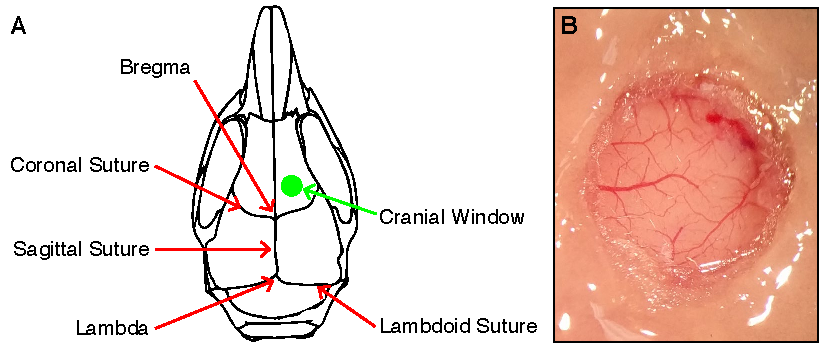
\includegraphics{figures/appendix_c/cranialwindow.pdf}
    \caption[Location of the cranial window on the mouse skull]{
        \label{fig:cranialwindow}
        Location of the cranial window relative to bregma. Skull illustratrion adapted from \cite{Cook:1965wb}.
    }
\end{figure}

The scalp was shaved and resected to expose skull between the bregma and lambda cranial coordinates. A thin layer of cyanoacrylate (Vetbond Tissue Adhesive, 3M) was applied to the exposed skull to facilitate the adhesion of dental cement during a later step. A 2-3 mm diameter portion of the skull over the frontoparietal cortex was removed while leaving the dura intact using a dental drill (0.8 mm burr, Ideal Microdrill, Fine Science Tools) with regular ACSF perfusion to prevent overheating. A 5 mm round cover glass (\#1.5, World Precision Instruments) was placed over the exposed brain and a dental cement mixture was deposited along the perimeter while applying gentle pressure to the cover glass. This process bonded the cover glass to the surrounding skull to create a sterile, air-tight seal around the craniotomy and allowed for restoration of intracranial pressure. A second layer of cyanoacrylate was applied over the dental cement to further seal the cranial window. The medial and anterior edges of the window were approximately 2 mm rostral from bregma and 0.5 mm lateral from the sagittal suture (Figure \ref{fig:cranialwindow}). Animals were allowed to recover from anesthesia and monitored for cranial window integrity and normal behavior for at least two weeks prior to imaging. Additional carprofen injections (5 mg/kg) were administered subcutaneously two, four, and seven days post-surgery to relieve inflammation from the procedure.


%%%%%%%%%%%%%%%%%%%%%%%%%%%%%%%%%%%%%%%%%%%%%%%%%%%%%%%%%%%%%%%%%%%%%%%%%%%%%%%
% Section B.2 - Headbar Attachment
%%%%%%%%%%%%%%%%%%%%%%%%%%%%%%%%%%%%%%%%%%%%%%%%%%%%%%%%%%%%%%%%%%%%%%%%%%%%%%%
\section{Headbar Attachment} \label{app:headbar_attachment}

Animals designated for awake imaging underwent an additional procedure during the application of dental cement to permanently attach a metal headbar used for head fixation. The circular cutout in the headbar was aligned with the cranial window and rotated laterally until parallel with the cover glass. This ensured that the cranial window would be perpendicular to the imaging system's optical axis when the animal was restrained in the awake imaging setup. Dental cement was applied around the headbar to permanently attach it to the animal's skull.


%%%%%%%%%%%%%%%%%%%%%%%%%%%%%%%%%%%%%%%%%%%%%%%%%%%%%%%%%%%%%%%%%%%%%%%%%%%%%%%
% Section B.3 - Chronic Animal Maintenance
%%%%%%%%%%%%%%%%%%%%%%%%%%%%%%%%%%%%%%%%%%%%%%%%%%%%%%%%%%%%%%%%%%%%%%%%%%%%%%%
\section{Chronic Animal Maintenance}

Animals were checked daily to monitor both behavior and the integrity of the cranial window by veterinary staff at the University of Texas at Austin Animal Research Center (ARC). Animals were housed in climate-controlled rooms with timed lighting (12-hour light/dark cycles) to maintain a comfortable living environment and given food and water \textit{ad libitum}. Social housing with multiple animals reduced the risk of overeating commonly seen when solo housing animals. This minimized possible growth in the animal's size and helped maintain the integrity of the cranial window. Any aggression resulted in the removal of the aggressor into a separate cage.

After several weeks of recovery, animals were used for both acute and chronic imaging experiments. Cranial windows were lightly cleaned prior to each imaging session using a cotton swab and 70\% ethanol (v/v). If necessary, a topical application of mineral oil was used to improve image quality by index matching. Any discoloration on or around the cranial window was documented and monitored for possible infection. Any cracks in or breaking of the cranial window were also documented and resulted in the immediate euthanasia of the animal.


%%%%%%%%%%%%%%%%%%%%%%%%%%%%%%%%%%%%%%%%%%%%%%%%%%%%%%%%%%%%%%%%%%%%%%%%%%%%%%%
% END Appendix B
%%%%%%%%%%%%%%%%%%%%%%%%%%%%%%%%%%%%%%%%%%%%%%%%%%%%%%%%%%%%%%%%%%%%%%%%%%%%%%%



\chapter{Lerma's Appendix}
\index{Appendix!Lerma's Appendix@\emph{Lerma's Appendix}}%
The source \LaTeX{} file for this document is no longer quoted in
its entirety in the output document. A \LaTeX{} file can 
include its own source by using the command
\cn{verbatiminput\{\cn{jobname}\}}.


%%%%%%%%%%%%%%%%%%%%%%%%%%%%%%%%%%%%%%%%%%
\chapter{My Appendix \#2}
\index{Appendix!My Appendix \#2@\emph{My Appendix \#2}}%
\section{The First Section}
This is the first section.
This is the second appendix.

\section{The Second Section}
This is the second section of the second appendix.

\subsection{The First Subsection of the Second Section}
This is the first subsection of the second section of the second appendix.

\subsection{The Second Subsection of the Second Section}
This is the second subsection of the second section of the second appendix.

\subsubsection{The First Subsubsection of the Second Subsection of
		the Second Section}
This is the first subsubsection of the second subsection of the
second section of the second appendix.

\subsubsection{The Second Subsubsection of the Second Subsection
		of the Second Section}
This is the second subsubsection of the second subsection of the
second section of the second appendix.

%%%%%%%%%%%%%%%%%%%%%%%%%%%%%%%%%%%%%%%%%%
\chapter{My Appendix \#3}
\index{Appendix!My Appendix \#3@\emph{My Appendix \#3}}%

\section{The First Section}
This is the first section.
This is the third appendix.

\section{The Second Section}
This is the second section of the third appendix.





%%%%%%%%%%%%%%%%%%%%%%%%%%%%%%%%%%%%%%%%%%%%%%%%%%%%%%%%%%%%%%%%%%%%%%
% Bibliography
%%%%%%%%%%%%%%%%%%%%%%%%%%%%%%%%%%%%%%%%%%%%%%%%%%%%%%%%%%%%%%%%%%%%%%
\bibliographystyle{unsrt}
\bibliography{bibliography.bib}


%%%%%%%%%%%%%%%%%%%%%%%%%%%%%%%%%%%%%%%%%%%%%%%%%%%%%%%%%%%%%%%%%%%%%%
% Vita
%%%%%%%%%%%%%%%%%%%%%%%%%%%%%%%%%%%%%%%%%%%%%%%%%%%%%%%%%%%%%%%%%%%%%%
\begin{vita}
Colin Tan Sullender was born in Birmingham, Alabama in 1988 to Wayne Sullender and Thuan Hong Tan. He graduated from Homewood High School in Homewood, Alabama in 2007. He pursued a Bachelor of Science in bioengineering at the University of Washington in Seattle and graduated in 2011 with College Honors in Bioengineering. As an undergraduate, he worked as a research assistant in the laboratory of Dr. Wendy E. Thomas. He began his doctorate in biomedical engineering at The University of Texas at Austin in 2011 in the laboratory of Dr. Andrew K. Dunn working on the development of novel optical imaging systems for studying ischemic stroke. He completed his Master of Science in Engineering in biomedical engineering in 2016 and completed his doctoral degree in August 2018.
\end{vita}


%%%%%%%%%%%%%%%%%%%%%%%%%%%%%%%%%%%%%%%%%%%%%%%%%%%%%%%%%%%%%%%%%%%%%%
% END DOCUMENT
%%%%%%%%%%%%%%%%%%%%%%%%%%%%%%%%%%%%%%%%%%%%%%%%%%%%%%%%%%%%%%%%%%%%%%
\end{document}
